\RequirePackage{luatex85}
\documentclass[
version=3.28,  % KOMA-Script version
a4paper,
11pt,
twoside,
openright,
cleardoublepage=empty,
%headsepline,
%bibliography=totoc,  % don't use! This is managed by biblatex!
BCOR=10mm,
%DIV=calc,
%DIV=classic,
DIV=12,
%tablecaptionabove,
%headinclude=false, % makes the upper margin a bit smaller
footinclude=false,
chapterprefix,
appendixprefix,
%numbers=noenddot,
%draft,
final,
%noonelinecaption,
%abstracton,
%pointlessnumbers, % when using \appendix, points appear mysteriously
%usegeometry=true,% make typearea play well with geometry
]{scrbook}

\title{Describing Three-Dimensional Movements in an Audio Scene Authoring Format}
\author{Matthias Geier}
\date{Juni 2023}

\usepackage{colorprofiles}
\usepackage[a-2u,mathxmp]{pdfx}

%\usepackage{showkeys}

\usepackage{scrhack}

% for getting smaller margins in the appendix with \newgeometry:
%\usepackage{geometry}

% Load Sphinx stuff first, some things will be changed further down

\ifdefined\pdfimageresolution \pdfimageresolution= 96\relax\fi

\catcode`^^^^00a0\active\protected\def^^^^00a0{\leavevmode\nobreak\ }

\usepackage[booktabs]{sphinx}
\sphinxsetup{
%verbatimwrapslines=false,
%verbatimhintsturnover=false,
div.note_border-TeXcolor={HTML}{E0E0E0},
div.note_border-width=0.5pt,
div.note_box-decoration-break=slice,
div.warning_border-TeXcolor={HTML}{E0E0E0},
div.warning_border-width=1.5pt,
div.warning_background-TeXcolor={HTML}{FBFBFB},
div.warning_box-decoration-break=slice,
div.topic_box-shadow=none,
div.topic_border-TeXcolor={HTML}{E0E0E0},
div.topic_border-width=0.5pt,
div.topic_box-decoration-break=slice,
}
\fvset{fontsize=\small}% Jupyter code size

\usepackage{nbsphinx}

\usepackage{fancyhdr}% This is used by Sphinx anyway
\pagestyle{fancy}
\fancyhead[LE,RO]{\thepage}
\fancyhead[RE]{\textsl{\nouppercase{\leftmark}}}
\fancyhead[LO]{\textsl{\nouppercase{\rightmark}}}
\fancyfoot{}
\renewcommand{\headrulewidth}{0pt}
\fancypagestyle{plain}{\fancyhf{}}

% Restoring the default that has been overwritten by Sphinx.
% \setparsizes is recommended by KOMA-Script instead of \parindent and \parskip:
\setparsizes{1em}{0pt plus 1pt}{0pt plus 1fil}

% This is *not* recommended by the KOMA-Script docs, but I want a smaller bottom margin:
\addtolength{\textheight}{2cm}

\usepackage{polyglossia}
\setmainlanguage{english}
\setotherlanguage{german}

\usepackage{fontspec}
\usepackage{mathpazo}
\linespread{1.05}  % see http://www.tug.dk/FontCatalogue/urwpalladio/
\setmainfont{TeX Gyre Pagella}[Numbers=OldStyle]
\setmonofont{Latin Modern Mono Light}[Numbers=Lining]

% don't use \sffamily:
\setkomafont{disposition}{\normalcolor\bfseries}
\setkomafont{descriptionlabel}{\bfseries}

% no "inline" paragraph headings
\RedeclareSectionCommand[
beforeskip=-10pt,
afterskip=1sp,
]{paragraph}

% remove indentation form subparagraph
\RedeclareSectionCommand[
%runin=true,
%afterskip=1em,
indent=0pt,
]{subparagraph}

% bold math
\usepackage{bm}
\usepackage{mathrsfs}  % for \mathscr{}

%%% suppress widows and orphans
\widowpenalty=10000
\clubpenalty=10000
\displaywidowpenalty=10000 % before and after display-math

%\KOMAoption{DIV}{current}  % re-calculate after specifying main font

\usepackage{tikz}
\usetikzlibrary{
bending,
%calc,
chains,
graphs,
positioning,
quotes,
shapes.geometric,
shapes.symbols,
shapes.misc,
arrows.meta,
shadows,
}

\tikzset{
%minimum height=2em,
node distance=1em,
outer sep=auto,
every node/.style={align=center},
terminal/.style={rounded rectangle, draw},
process/.style={rectangle, draw},
document/.style={tape, tape bend top=none, draw},
database/.style={cylinder, shape border rotate=90, aspect=0.15, draw},
multiple/.style={double copy shadow, fill=white},
>=Stealth[bend],
shorten >=1pt,
}
\tikzgraphsset{
grow right sep,
%branch down sep,
nodes=draw,
}

% see https://tex.stackexchange.com/a/609248/
\tikzset{execute at end node=\strut}
\makeatletter
\def\tikz@align@newline{\strut\pgfutil@protect\tikz@align@newline@}
\makeatother

% bigger integral and summation signs for fonts 11pt and 12pt
\usepackage{exscale}

\usepackage[titletoc,toc]{appendix}
% workaround to get a slightly bigger space before appendices in toc
\renewcommand{\appendixtocname}{\mbox{}\vfill\mbox{}}
\noappendicestocpagenum

\usepackage{fancyref} % cool references (\fref and \Fref)
% uses varioref internally

\newcommand{\ie}{i.\,e.\ }
\newcommand{\eg}{e.\,g.\ }

\usepackage[intlimits]{amsmath}
%% intlimits: integral range above and below
\usepackage{amssymb}
\usepackage{amstext}
\usepackage{nicefrac}

% the package "caption2" is obsolete!

\addtokomafont{caption}{\small\itshape}
\addtokomafont{captionlabel}{\bfseries}
\setcapindent{0pt}
\setlength{\abovecaptionskip}{0pt}
\setlength{\belowcaptionskip}{0pt}
\setcapwidth{.9\textwidth}

%\counterwithin{figure}{chapter}
%\renewcommand{\thefigure}{\arabic{chapter}.\arabic{figure}}

\usepackage{siunitx}

\newcommand{\code}[1]{\texttt{#1}}

\usepackage{graphicx}
\usepackage{hyperref}
\hypersetup{
pdfencoding=unicode,
pdfpagemode=UseNone,
pdfstartview=FitH,
breaklinks=true,
bookmarks=true,
% appendices are uppercase for the pdf chapters and lowercase (sc) in the
% document. see beginning of appendix.
bookmarksnumbered=true,
%bookmarksdepth=5,
%hyperindex=false,
bookmarksopen=false,
hidelinks,
%colorlinks,
%linkcolor=,citecolor=,urlcolor=,
pdfsubject={audio scene description},
pdfkeywords={ASDF, SSR},
}
\pdfcompresslevel=9
% Fix anchor placement for figure captions (must be loaded after hyperref)
\usepackage{hypcap}

\usepackage{csquotes}  % recommended by biblatex
\usepackage[
backend=biber,
style=authoryear-comp,
]{biblatex}  % see biblatex.cfg for further options

\addbibresource{geier_dissertation_2024.bib}
\addbibresource{sphinx-splines/splines/doc/references.bib}
%\DeclareDelimFormat{nameyeardelim}{\addcomma\space}

\newcommand*{\mychapterformat}[1]{%
\hfill\chapappifchapterprefix{\ }\raisebox{-.4\baselineskip}[0pt][0pt]{%
\scalebox{4}{\rmfamily#1\thechapter\autodot}}%
%\setlength{\baselineskip}{0pt}%
\\[-.7\baselineskip]%
%\vspace{.3\baselineskip}%
\textcolor{white}{\rule{\textwidth}{.5mm}}\\[-\baselineskip]%
\vspace{2mm}
\textcolor{white}{\rule{\textwidth}{.5mm}}\\[-\baselineskip]%
\vspace{2mm}
\textcolor{white}{\rule{\textwidth}{.5mm}}%
}
\renewcommand*{\chapterformat}{\mychapterformat{\itshape}}
\usepackage{relsize} % for the \relsize command
\newcommand{\SecNumFont}{\mdseries\rmfamily\scshape\relsize{1.5}}
\renewcommand*{\othersectionlevelsformat}[1]{%
  \SecNumFont\csname the#1\endcsname\autodot\enskip}
%\newcommand{\mynumberline}{}
%\let\mynumberline\numberline
%\renewcommand{\numberline}[1]{\mynumberline{\SecNumFont#1}}
%% pagenumber of chapters in TOC
%\newcommand{\mycontentsline}{}
%\let\mycontentsline\contentsline
%\renewcommand{\contentsline}[3]{\mycontentsline{#1}{#2}{\rmfamily#3}}

\setcounter{tocdepth}{4}
\setcounter{secnumdepth}{4}

\addtokomafont{chapter}{\let\raggedsection\raggedleft}

\hyphenation{
Be-schrei-bung
Au-dio-BIFS
allow
allows
param-e-ter-i-za-tion
co-ordi-nates
}

\usepackage[
type={CC},
modifier={by},
version={4.0},
imagewidth=7em,
]{doclicense}

\begin{document}

\makeatletter
\let\thetitle\@title
\let\theauthor\@author
\let\thedate\@date
\makeatother

\begin{titlepage}
  \begin{center}
    \vspace*{\fill}
    \textbf{\huge\thetitle}
    \vfill
    \normalsize


\begin{german}
Dissertation\\
zur Erlangung des akademischen Grades\\
Doktor-Ingenieur (Dr.-Ing.),\\
der Fakultät für Informatik und Elektrotechnik\\
der Universität Rostock\\
vorgelegt von\\
\theauthor, geb. am 12.\,Feb.\,1979 in Salzburg.
\end{german}
  \end{center}
    \vfill
\begin{german}
Rostock, \thedate
\end{german}

\vskip2\baselineskip

\doclicenseThis
\end{titlepage}

\newpage
\vspace*{\fill}
\noindent
\textbf{Gutachter:}\\
Prof.\ Dr.-Ing.\ Sascha Spors, Universität Rostock\\
Prof.\ Dr.-Ing.\ Thomas Sporer, Universität der Künste Berlin\\
Prof.\ Dr.-Ing.\ Alexander Raake, TU Ilmenau
\vskip\baselineskip
\noindent
\textbf{Jahr der Einreichung:} 2023\\
\textbf{Jahr der Verteidigung:} 2024

\frontmatter

\cleardoubleoddpage
\vspace*{\fill}
\thispagestyle{empty}
{ \renewcommand*{\raggedsection}{\centering}

\addsec*{\abstractname}
After a brief historic overview
about \emph{spatial audio reproduction},
the concept of \emph{object-based} audio reproduction is explained
and the need for \emph{spatial audio scenes} is stated.
Several existing formats for describing object-based audio scenes
are reviewed,
with special focus on the description of 
movement of scene objects over time.
A new scene authoring format named
Audio Scene Description Format (ASDF) is presented.
Its description of movement of scene objects
is based on several types of \emph{splines},
which are thoroughly investigated, both for position and for rotation.
Finally, an open-source ASDF library implementation
and two integrations of this library
are presented, which make it possible for everyone to try the ASDF right now.

\vfill
\begin{german}
\addsec*{\abstractname}
Nach einem kurzen Abriss über die Geschichte
der \emph{räumlichen Audiowiedergabe}
wird das Konzept der \emph{objektbasierten} Audiowiedergabe erklärt
und die Notwendigkeit von \emph{räumlichen Audioszenen} wird festgestellt.
Einige existierende Beschreibungsformate für
objektbasierte Audioszenen werden betrachtet,
mit Hauptaugenmerk auf die Beschreibung der Bewegung von Szenenobjekten
im Zeitverlauf.
Ein neues Format für Szenenautoren namens
Audio Scene Description Format (ASDF) wird präsentiert.
Seine Beschreibung der Szenenobjektbewegungen fußt auf
mehreren Arten von \emph{Splines},
die gründlich untersucht werden,
sowohl für Position als auch für Rotation.
Zu guter Letzt wird die Implementierung
einer quelloffenen ASDF Softwarebibliothek sowie zwei Einbindungen dieser
Bibliothek präsentiert,
die es ab sofort jedem ermöglichen, das ASDF auszuprobieren.

% vim: spelllang=de


\end{german}
} % end of raggedsection == centering
\vfill
\cleardoubleoddpage

\tableofcontents

\mainmatter

\renewcommand{\dictumwidth}{0.5\textwidth}
\setchapterpreamble[ol][0.5\textwidth]{%
\dictum[\cite{garity1941fantasound}]{%
It has been found that
by artificially causing the source of sound
to move rapidly in space
the result can be highly dramatic and desirable.}}

\addchap{Introduction}

The goal of \emph{spatial audio reproduction}
is to create auditory events for a listener or multiple listeners,
which are perceived as arriving from specific spatial directions.
This can be achieved either with headphones or with arrangements
of multiple loudspeakers.
Such technology can be used,
for example,
for creating
spatial music performances,
audio plays
or spatial sound tracks for movies.

To set everything into perspective, chapter~\ref{sec:history}
will give an overview about the historic development of spatial audio
reproduction and present some old and new techniques
for creating spatial audio experiences for an audience.
This is also where the term \emph{channel-based} will be introduced
to classify reproduction systems
where each loudspeaker driving signal
is stored and distributed in its own separate channel.
This will be contrasted with
the term \emph{object-based},
which represents a whole new reproduction paradigm.
Instead of delivering an \emph{audio mix} which is tied to a fixed loudspeaker
setup (or to two headphone channels),
a so-called \emph{audio scene} comprised of individual sound sources is
created which holds all source signals as well as additional data like source
positions and other scene parameters.
Based on such an audio scene,
the loudspeaker or headphone signals are generated in real time
for any given reproduction setup.

Chapter~\ref{sec:existing-formats}
will describe some existing file formats to store object-based
audio scenes.
The main focus will be on the handling of three-dimensional movements
of scene objects.
Most of those formats were not explicitly designed for authoring,
and even though many formats are text-based,
their syntaxes make it unnecessarily hard to author scenes by hand.
Most formats do not provide any
high-level \emph{declarative}\footnote{%
For an explanation of the term \emph{declarative} see
section~\ref{sec:declarative-procedural-sampled}.}
syntax for the description of smooth movements.

The Audio Scene Description Format (ASDF)
-- a new authoring format for object-based audio scenes --
will be presented in chapter~\ref{sec:format-development}.
Instead of using spatial relationships as the main structural element,
it uses temporal relationships.
Elements of a scene can happen in parallel or in sequence.
By nesting so-called \emph{time containers},
arbitrary time relationships can be defined.
Both audio clips and the \emph{transforms} that control their spatial
positions and movements
are part of the same timeline.
Spatial relations are still very important,
but they are not defined by the top-level file structure.
Instead, spatial relationships have to be explicitly established
by referencing other scene objects or transforms via their IDs.

A detailed description of all features of the ASDF
is available in appendix~\ref{sec:asdf},
which also includes a lot of small examples.
The \emph{declarative}
definition of movements of objects in a scene
-- including the rotation of objects and groups of objects --
is based on \emph{splines}.
An extensive review of all the relevant types of splines
is provided in appendix~\ref{sec:splines}.
The appendices are an integral part of this thesis
and they should not be overlooked.
The reason why those two appendices are not part of the main text
is that they are actually self-contained projects,
which are separately available online.
Furthermore,
they are meant to evolve beyond being used as part of this thesis.
Appendix~\ref{sec:splines} not only illustrates
the properties of all the types of splines used in the ASDF,
but it also provides tools for investigating further types
and maybe developing new types.
It thoroughly derives the fundamentals of interpolatory polynomial splines
in Euclidean space and it applies the same methods
-- as far as possible -- to rotation splines.
Three-dimensional rotation splines are notoriously hard to visualize
and since this thesis is printed on paper,
only sequences of snapshots of rotations can be shown.
However,
in the online
HTML version\footnote{\url{https://splines.readthedocs.io/}},
a number of animations are available that can much better
illustrate the behavior of subtly different rotation splines.

It is an important goal of this thesis
to not only define a theoretical file format on paper,
but also to enable its practical usage
in order to be able to properly evaluate its capabilities and weaknesses.
Therefore, an open-source software library has been implemented,
which is described in chapter~\ref{sec:implementation}.
This library has also been integrated in a stand-alone
software for spatial audio reproduction,
which means that the ASDF is ready to be tried out by anyone who is interested.


\addsec{Acknowledgements}

I would like to thank Sebastian Möller,
head of the Quality and Usability (QU) Lab,
Technische Universität Berlin\footnote{\url{https://www.tu.berlin/qu/}},
for taking me in as a PhD student
and for giving me all the support I could wish for
during the time I worked there.
I am indebted to Sascha Spors,
at the time head of the spatial audio group at QU Lab and later professor
at the Institute of Communications Engineering at Universität
Rostock\footnote{\url{https://www.int.uni-rostock.de/}}
for acting as my thesis advisor since the beginning
and for his support over all those years.
Thanks to Jens Ahrens
for introducing me to the QU Lab in the first place
and for his continuous collaboration on the \emph{SoundScape Renderer}
which now serves as a proving ground for the ASDF.
Thanks to all my colleagues at QU Lab in Berlin
and at the Institute of Communications Engineering in Rostock
for many fruitful discussions
and for contributing to a great working experience.
I would like to thank Jürgen Herre
for helping me find the motivation to finally finish this thesis.
A big thank you goes to
Tracy Harris for proofreading the whole text including the appendices.
Thanks to Mikhail Korotiaev for several suggestions
for improvements in appendix~\ref{sec:splines}.
Finally, I would like to thank all the
maintainers and contributors of the many open-source software projects
that were used for creating this thesis and the associated software and
documentation: \LaTeX, Sphinx, Jupyter, Matplotlib, NumPy, SymPy,
Python and Rust, just to name a few.
Specifically, I would like to thank
Jean-François B.\footnote{\url{https://github.com/jfbu}}
for his work on the \LaTeX\ output of
\emph{nbsphinx}\footnote{\url{https://nbsphinx.readthedocs.io/}},
without which the Jupyter code cells in the appendix would look much
less pleasing.


\chapter{Spatial Audio From the Beginning}
\label{sec:history}

There were sound waves in the early universe,
as can be observed today via
\emph{baryon acoustic oscillations}%
\footnote{\url{https://en.wikipedia.org/wiki/Baryon_acoustic_oscillations}},
and since that era there have been -- and still are -- many places in the universe
which are filled with an elastic medium that allows sound propagation.
This chapter will focus on sound waves in the atmosphere of planet Earth.
However, any sound travelling
through any medium that inhabits any three-dimensional space
can be considered \emph{spatial sound}.

The terms \emph{spatial sound} and \emph{spatial audio}
can be used interchangeably.
Etymologically, the term \emph{audio},
which is the first-person singular form of the verb \emph{audire}
-- Latin for \emph{hearing/listening} --
implies a sentient being capable of auditory perception
(and, strictly speaking, with Latin language skills)
actually hearing the sound.

Even before life existed on Earth,
its atmosphere (and its oceans as well) must have carried spatial sound,
caused, for example, by storms, meteor strikes or volcanic eruptions
(see figure~\ref{fig:no-observer}).

\begin{figure}[htbp]
\centerline{\tikz \graph {
no initiator [terminal, dotted, font=\itshape] -> [dotted]
natural occurrence -> [dotted]
no observer [terminal, dotted, font=\itshape]
};}
\caption{Spatial sound produced by inanimate processes in a lifeless medium}
\label{fig:no-observer}
\end{figure}

Animals first evolved and diversified in the oceans,
where many of them developed an auditory sense.
When the first animals migrated to land,
they adapted their spatial hearing capabilities
to the new atmospheric medium
or developed entirely new auditory mechanisms.
The development of hearing -- especially spatial hearing --
certainly was (and still is) a very helpful tool for the survival of a species.
It can help predators find prey,
but it can also help prey evade predators
(see figure~\ref{fig:predator-prey}).

\begin{figure}[htbp]
\centerline{\tikz \graph {
"predator" [terminal] -> attack -> potential prey [terminal]
};}
\caption{Spatial sound unintentionally produced by a predator}
\label{fig:predator-prey}
\end{figure}

Apart from sound as an accidental
by-product of locomotion and bodily functions,
animals have developed a wide variety of ways to actively create sounds,
serving a multitude of purposes.
Spatial sound can help finding a mate,
localizing one's own offspring in an overcrowded breeding colony
and in general with intra- and inter-species communication.
In addition to mammals,
several classes of animals are known to be capable of spatial hearing,
like
fish \parencite{popper1993fish},
birds \parencite{macleod2006emu,konishi2003coding}
and even insects \parencite{yager1999structure,schmidt2011cocktail}.
A notable exception is the \emph{praying mantis},
which has an acoustic sense but only a single ear,
making it an \emph{auditory cyclops}
which can most likely not differentiate between
different angles of sound incidence \parencite{yager1986cyclopean}.

Whenever an individual produces sound
and another individual (or even the same one)
perceives it in a way that spatial information is conveyed,
we can consider it a \emph{spatial audio performance}
(see figure~\ref{fig:basic-performance}).

\begin{figure}[htbp]
\centerline{\tikz \graph {
"performer" [terminal] -> performance -> consumer [terminal]
};}
\caption{Spatial audio performance}
\label{fig:basic-performance}
\end{figure}

Like all diagrams in this section, the diagram in
figure~\ref{fig:basic-performance}
is simplified.
There can be multiple performers working together,
but there can also be multiple performances
coalescing into a single experience for a consumer.
There can be multiple consumers, often called an \emph{audience}
(which happens to have the same Latin root as the term \emph{audio}).
There can be feedback from consumers that influences the performance and
consumers may themselves create spatial sound
in form of applause or other audible reactions.
The spatial audio performance
can of course be part of a multi-sensory performance.

Not only the words \emph{performer} and \emph{consumer},
but also the term \emph{performance} itself are used very loosely here.
The performance could simply be the act of communicating
between two animals, including humans.
The auditory and spatial aspect thereof would be covered by the field of
communication acoustics
\parencite{blauert2005communication,pulkki2015communication}.
Instead of (or in addition to) communication,
the goal of the performance could also simply be entertainment.
Whether a performance is artistic or accidental
or anything in between,
here we are interested in the spatial audio aspect of it.

Many animals are capable of spatial audio performances,
but as far as we know,
only humans can write down instructions for others to perform their ideas
(see figure~\ref{fig:performance-with-instructions}).

\begin{figure}[htbp]
\centerline{\tikz \graph {
"creator" [terminal] ->
instructions [document] ->
performance ->
consumer [terminal]
};}
\caption{Spatial audio performance based on written instructions}
\label{fig:performance-with-instructions}
\end{figure}

Of course not every detail of the performance
can be controlled by written instructions,
and performers will have a lot of leeway in interpreting those instructions.
For example, listening to the performance of an ancient Greek tragedy
in an amphitheater
was certainly very much a spatial audio experience,
but the control of spatial audio aspects of the performance
via written stage directions was limited.

Not only theater, but also
traditional musical performances have an inherent spatial component.
An early example for consciously using spatial properties in musical pieces is
the polychoral practice from 16\textsuperscript{th} century Venice,
where multiple choirs are instructed to perform from different places within a
venue, most famously in the \emph{Basilica San Marco di Venezia}.
In modern literature,
this is often referred to as \emph{cori spezzati},
but this term was probably not used at the time
\parencite{bryant1981cori,gembicki2020cori}.

Some classical and romantic operas and symphonies contain short parts
for a separate group of off-stage musicians
-- often positioned outside the main hall --
to achieve an effect of great spatial distance.
Some compositions require
spatially separated groups of musicians
(like
\emph{Notturno in D, K.\,286} by Wolfgang Amadeus Mozart and
\emph{Symphony No.~4} by Charles Ives)
or even multiple full orchestras
(like \emph{Gruppen} by Karlheinz Stockhausen).

The performances described so far were originally intended
to be performed for an audience
located in the same room
as the performers or
-- in case of open air performances --
in the same outdoor area.
With the invention of the \emph{telephone} around 1860,
it became possible to
transmit sound over an electrical wire and listen to it at the far end.
This way, it was possible to listen to an audio performance
without being anywhere near the performers
(see figure~\ref{fig:telephone-transmission}).

\begin{figure}[htbp]
\centerline{
\tikz \graph {
"creator" [terminal] ->
instructions [document] ->
performance ->
"transmission\\via telephone" ->
consumer [terminal]
};}
\caption{Transmitted audio performance}
\label{fig:telephone-transmission}
\end{figure}

The \emph{phonograph} -- invented in 1877 --
allowed to store the recording of an audio performance
(originally in grooves of varying depth on a wax cylinder)
and to reproduce it at a later time
(see figure~\ref{fig:mono-recording}).

\begin{figure}[htbp]
\centerline{\tikz \graph {
"creator" [terminal] ->
instructions [document] ->
performance ->
"phonograph\\recording" [database] ->
reproduction ->
consumer [terminal]
};}
\caption{Recorded audio performance}
\label{fig:mono-recording}
\end{figure}

Even though those inventions were certainly groundbreaking,
the poor sound quality (compared to today's standards) and
the use of only a single audio channel
severely limited the perception of spatial aspects of the performance.
In 1881,
Cl\'ement Ader presented his
\emph{th\'e\^atrophone}
at the \emph{International Exposition of Electricity} in Paris
\parencite{hospitalier1881auditions}.
Instead of a single transmission channel, it used two telephone mouthpieces
mounted on the left and right side of the stage of \emph{Opéra Garnier},
connected with two separate telephone lines to two earpieces
(located in a different building in Paris),
which allowed listening to the performances happening on the stage,
including some crude spatial perception of the performers' positions.
The original installation was able to accommodate multiple listeners at once,
each one using a separate pair of mouthpieces,
telephone lines and earpieces.
A
patent\footnote{\url{https://worldwide.espacenet.com/patent/search?q=US257453A}}
was granted in 1882.
In 1890, the system was established as a commercial service
which was in operation until 1932.

The th\'e\^atrophone
had shown the advantages of using two channels instead of one,
but since no amplifiers were available at the time,
applications were limited.
In the following decades,
further development of microphones, amplifiers and loudspeakers
opened up more possibilities.
In 1924, Franklin M. Doolittle was granted a
patent\footnote{\url{https://worldwide.espacenet.com/patent/search?q=US1513973A}}
suggesting the transmission of left and right audio signals
over two separate AM radio channels.
Doolittle also made experimental broadcasts from his
radio station WPAJ in New Haven, Connecticut
\parencite{doolittle1925binaural}.
In his studio,
two microphones with a center-to-center distance of
about \qty{18}{\centi\meter} were used to pick up sound.
The two signals were broadcast over two separate radio frequencies
and listeners had to use separate AM receivers for each frequency.
The distance between microphones was based on the distance between human ears
and broadcasts were mainly intended for headphone reproduction.
In a
patent\footnote{\url{https://worldwide.espacenet.com/patent/search?q=US1624486A}}
from the year 1927,
Harvey Fletcher and Leon Sivian
suggest the use of an artificial head containing two microphones near the ears
to simulate the acoustic scattering of a real human head which
strongly affects spatial perception.
\textcite{fletcher1933illusion}
describes a realization of this idea in the form of
an acoustic manikin named \emph{Oscar}.

\begin{figure}[htbp]
\centerline{\tikz \graph {
"creator" [terminal] ->
instructions [document] ->
performance ->
"two-channel\\recording" [database] ->
"binaural\\reproduction" ->
consumer [terminal]
};}
\caption{Binaural recording of a spatial audio performance}
\label{fig:binaural-recording}
\end{figure}

Just as sound \emph{transmission} was extended to more than one channel,
sound \emph{recording} followed suit
(see figure~\ref{fig:binaural-recording}).
Another
patent\footnote{\url{https://worldwide.espacenet.com/patent/search?q=US1817177A}}
by Doolittle
-- published in 1931 but filed already in 1921 --
describes how two channels can be stored on a phonograph record
with two grooves running side by side.
The tonearm would have two needles next to each other
to reproduce the left and right signals.
A very similar approach is described in a 1924
patent\footnote{\url{https://worldwide.espacenet.com/patent/search?q=US1508432A}}
by
Harry Wier (also filed in 1921).
A 1932
patent\footnote{\url{https://worldwide.espacenet.com/patent/search?q=US1855149A}}
by W.\ Bartlett Jones (filed in 1927)
mentions multiple variations of two-channel phonographs,
including one using a record with
a single groove with variations in both depth and lateral shift.
This was later known as \emph{V/L} for \emph{vertical/lateral}.
Alan Dower Blumlein's UK
patent\footnote{\url{https://worldwide.espacenet.com/patent/search?q=GB394325A}}
from 1933 (filed in 1931)
suggests rotating the single groove recording apparatus by 45 degrees,
so that the variations of the two channels
still happen at an angle of 90 degrees to each other,
but at 45 degrees relative to the disk surface.
This type of record is also known as \emph{45/45}.
A few years later,
the same \emph{45/45} approach was also proposed in a US
patent\footnote{\url{https://worldwide.espacenet.com/patent/search?q=US2114471A}}
submitted by Arthur Keller and Irad Rafuse.
The \emph{45/45} method is still used in today's vinyl records,
which are once again quite popular,
despite the abundance of modern digital storage media.

Most of the reproduction systems mentioned so far were mainly targeted for
headphone listening.
The goal was to
place two microphones at the same distance as between two ears
to create appropriate phase differences.
Ideally, some kind of dummy head was used
to model the acoustic shadow of a real head.
Since the two signals are meant to be reproduced very close to
the two ears of a listener, respectively,
this method is called \emph{binaural} reproduction,
after the Latin words \emph{bis} and \emph{auris},
which mean \emph{two times} and \emph{ear}.
An overview of the history of binaural recording technology can be found in
\parencite{paul2009binaural}.

The idea of using more than one channel was of course also applied to
loudspeaker-based reproduction.
This was especially relevant for movie theaters.
Even when commercial movies were still silent
(the first feature film with sound
-- \emph{The Jazz Singer} --
came out in the year 1927),
inventors were already thinking about multi-channel sound for movies.
A
patent\footnote{\url{https://worldwide.espacenet.com/patent/search?q=US1124580A}}
by Edward Amet (filed 1911, granted 1915)
describes a device that uses a mono phonograph recording
which is switched (not panned!) between multiple telephone receivers.
Loudspeaker technology was still in its infancy,
and apparently telephone receivers were state of the art
for sound reproduction.
The telephone receivers would be placed at different positions
close to the screen,
and the idea was that switching between them allowed the sound
to follow the corresponding actions shown on the screen,
or as it is phrased in the patent text,
``By the means shown a picture of a moving sound-making object
may be accompanied in its travel across the screen by its
appropriate reproduced sound.''
The switching of the signal was meant to be achieved by means of
electrically conducting lines mounted on small insulating plates
-- individually hand-crafted for each phonograph record used --
touching an electric contact point
which moves together with the tonearm of the phonograph.

In a
patent\footnote{\url{https://worldwide.espacenet.com/patent/search?q=US1589139A}}
from 1926,
Earl H.\ Foley
suggests using
a three-channel recording
reproduced over loudspeakers at the left and the right and behind the
center of the movie screen.
The sound track is to be recorded with three microphones
placed across the field of view when shooting the movie.
The goal is again for the sound to follow the movements
of the performers visible on screen.

Three channels were also used in 1933, when a performance of the
Philadelphia Symphony Orchestra
was picked up in the \emph{Academy of Music} in Philadelphia
with three microphones,
transmitted via three telephone lines
and reproduced in \emph{Constitution Hall} in Washington, D.\ C.,
with three loudspeakers.
The system and its capability for spatial audio reproduction
has been presented in a
\emph{Symposium on
Wire Transmission of
Symphonic Music and its
Reproduction in Auditory Perspective}.
The microphone and loudspeaker setup that was used in the two halls is shown in
\parencite{bedell1934auditory}.
\textcite{steinberg1934auditory} describe
additional speech localization experiments that have been conducted
with three loudspeakers
in the auditorium at the \emph{Bell Telephone Laboratories}
connected to three microphones in a smaller pick-up room.
Using only two channels instead of three still provided
good angular localization from a center listening position, albeit
with slightly less accurate depth perception.
As the observer moved to one side, however,
the virtual source shifted more rapidly toward the nearer loudspeaker
than in the three-channel setup.
They conclude that ``2-channel
reproduction of orchestral music gives good satisfaction, and the
difference between it and 3-channel reproduction for music probably
is less than for speech reproduction or the reproduction of sounds
from moving sources.''

A three-channel sound track was also used
in the first commercial feature-length movie with stereophonic sound
-- Walt Disney's \emph{Fantasia} -- which premiered in the year 1940.
The movie consists of
a series of classical music pieces, accompanied by animation sequences in
different styles.
One of the segments
features none other than Mickey Mouse
as the titular character in Paul Dukas's
\emph{Sourcerer's Apprentice}.
A narrator gives some explanations
in-between the segments,
and Mickey Mouse has a short conversation with Leopold Stokowski --
the conductor of the sound track --
but there is no spoken word during the music pieces
and there are no sound effects.
This means that any spatial audio positioning and movement
was only applied to the music,
which is not very common nowadays.

Most of the sound track was recorded in the
\emph{Academy of Music} in Philadelphia
onto
eight tracks of optical film.
Six tracks were used for recording different sections of the orchestra,
one track held a mono mix of those first six tracks
and one track contained a distant pick-up of the whole orchestra.
These tracks were afterwards mixed in a so-called
\emph{re-recording} process, resulting in three program audio channels
destined for the left, center and right loudspeakers, respectively.
To be able to dynamically distribute a single recorded track
between the three loudspeakers,
while at the same time keeping the total power constant,
a device nicknamed \emph{``The Panpot''} was used.
This name is still used today
and the whole process is nowadays called \emph{panning}.

Optical sound tracks at the time did not have enough dynamic range
to faithfully reproduce the sound of an orchestra.
To overcome this, three variable-gain amplifiers were used,
which were controlled by the amplitudes of three sine tones
at constant frequencies of \qty{250}{}, \qty{630}{} and \qty{1600}{\hertz},
respectively.
These control tones were generated in the aforementioned re-recording process
and were recorded onto a separate channel besides the three program channels.
The four channels were then printed on 35-mm film.
When \emph{Fantasia} was shown in movie theaters,
this film was played back in synchrony with a second film
containing the moving images.
The channel with the three control tones was fed into the
Tone-Operated Gain-Adjusting Device (TOGAD),
which in turn controlled the gain stages of the three amplifiers.
Those amplifiers were of course using vacuum tubes,
which was state of the art at the time.
The whole technology was called \emph{Fantasound}
\parencite{garity1941fantasound}.

Modern texts sometimes claim that
the TOGAD has also been used
for panning and even for moving sounds around the audience,
and some texts mention a relatively large number of loudspeaker channels.
With only three control tones and three input channels,
the panning options would have been very limited, though.
Therefore, we can infer that the control tones
were mostly used for increasing the dynamic range.
However,
in addition to the three main loudspeakers behind the projection screen,
there were indeed auxiliary loudspeakers placed in the auditorium.
But those were manually switched on by the projectionist
in the last segment of the movie -- \emph{Ave Maria} --
and they were fed by two of the main three sound channels.
In some of the installations,
the switching was automated by a mechanical relay system
operated by means of notches on the edge of the film.

The \emph{Fantasound} system
required a lot of equipment that was generally not available at cinemas.
Therefore, the movie was presented as a road-show only at selected cinemas,
where the custom equipment was installed temporarily.
Partly because of the large cost of these installations,
\emph{Fantasia} was not a big commercial success.
Another reason for discontinuing the project was the involvement of the US
in the Second World War.

At the time,
the terms \emph{stereophonic} and \emph{binaural}
were often used interchangeably.
However, \textcite{snow1953stereo} makes a clear distinction
between the terms as they are still used today:
\emph{binaural} recordings are made with two microphones
-- preferably in an artificial head --
and intended for headphone reproduction,
while \emph{stereophonic} recordings are made with two or more microphones
and intended for reproduction with two or more loudspeakers
``spaced in front of a listening area.''
It is important to note that even though two-channel recordings
were -- and still are -- very common,
stereophony is not limited to two channels at all.
The Greek word \emph{stereos} simply means \emph{firm} or \emph{solid}.
The term \emph{stereophonic} was most likely inspired
by \emph{stereoscopic} images and photographs \footnote{\url{%
https://en.wikipedia.org/wiki/Stereoscopy}},
which were all the rage
in the second half of the 19\textsuperscript{th} century.

After the Second World War,
magnetic tape was rapidly displacing
phonograph records and optical film as a recording medium and
in the 1950s,
tape recorders were also conquering the concert halls.
Electronic sounds and natural sounds were recorded on tape,
edited and often electronically modified.
Those tapes were then played back during a concert in a concert hall.
For example, the composition \emph{Williams Mix} by
John Cage, composed between 1951 and 1953,
was realized on eight heavily spliced mono tapes,
which were played back by eight separate tape machines
with eight equidistant loudspeakers around the audience.

Olivier Messiaen's composition \emph{Timbres-durées}
was first performed in 1952
from a four-track tape using four loudspeakers.
Two tracks were assigned to the left and right loudspeakers
in front of the audience.
Another track was played back over a loudspeaker behind the audience
and one mounted on the ceiling above the audience.
Finally, one special track called \emph{cinématique}
was interactively distributed over all four loudspeakers
using a
spatialization device
called
\emph{pupitre d'espace},
developed Jacques Poullin.
This device consisted of four rings of \qty{50}{\centi\meter} diameter
placed around the conductor,
representing the four loudspeaker positions left, right, above and towards the
rear end of the room.
The conductor was holding an electrical coil in his hand
and moving this coil with big gestures between the rings
made the sound move between the four loudspeakers
\parencite{battier2015discoveries}.

Another famous example is
the piece \emph{Kontakte} by Karlheinz Stockhausen
(composed 1958--60),
in which he used a rotation table on which a loudspeaker was mounted on and
which was manually rotated.
The resulting sound was recorded on
tape via four microphones at fixed positions around the table.
During a concert, the four-track tape was played back on four loudspeakers
around the audience.

The concept of playing tapes over loudspeakers
was taken to the next level
at the Philips Pavilion on the 1958 Brussels World's Fair.
Edgar Varèse composed a spatial music piece as part of
an eight-minutes-long multimedia spectacle
called \emph{Poème électronique},
involving a wardrobe-sized 3-track magnetic tape machine,
20 amplifiers and 350 loudspeakers
\parencite{kalff1958poem}.
The routing of the audio tracks to groups of loudspeakers,
as well as the control of illumination effects,
was facilitated by another magnetic tape machine,
running in synchrony with the first.
The second tape contained 15 tracks
with 12 fixed-frequency control signals per track.
Some of the continuous signals controlled relays to activate
certain loudspeaker groups,
others were used to select which of the three audio tracks to use
as input for those groups.
A part of the loudspeakers formed five so-called \emph{sound routes}
along the inside walls of the pavilion,
which created the illusion of moving sound sources.
A train of pulses in one of the control signals
was used to turn a rotary control to switch from one loudspeaker to the next.
The rate of these pulses -- up to 10 per second --
determined the speed of the apparent sound source.
In the following years,
many more spatial audio compositions for tape and loudspeakers were created,
for example
\emph{Bohor} (1962) by Iannis Xenakis
and
\emph{HPSCHD} (1969) by John Cage.

Visitors of the 1970 World's Fair in Osaka, Japan,
had the opportunity to experience
large-scale spatial music performances
in more than one custom-built pavilion on the same exhibition grounds.
The German Pavilion was a spherical building housing a spherical auditorium.
50 groups of loudspeakers were mounted at different heights,
surrounding a central listening platform from all directions,
including above and below.
Compositions by Stockhausen for
live soloists and multichannel tape
were performed with live spatialization.
During the performances,
the tracks could either be directly routed to fixed loudspeaker positions
or via two custom-built
\emph{rotation mills}
which could be used to move sounds
along trajectories of 10 loudspeaker groups each
by turning a hand crank
\parencite{bates2015kontakte}.

Another notable venue at the Osaka Expo in 1970 was the
\emph{Space Theatre}
in the
so-called \emph{Steel Pavilion} of the \emph{Japan Iron and Steel Federation},
where
Iannis Xenakis' composition \emph{Hibiki-Hana-Ma} was performed.
A 12-track tape was spatialized along elaborate trajectories
according to control commands
that were recorded on film.
The exact number of loudspeakers is unclear,
but maybe 264 groups of loudspeakers were installed in the pavilion,
with a total of 800 individual loudspeakers
\parencite{paland2015xenakis}.

While most of the compositions mentioned above were made
without the help of computers (Cage's \emph{HPSCHD} being a notable exception),
the use of computers became much more common in the 1970s.
The computer-generated signals, however,
were still often recorded on analog tapes to be used for the performances.
In 1972,
John Chowning composed the piece \emph{Turenas},
which was to be played on
four loudspeakers placed in the corners of a square.
Both the sound synthesis
-- using the recently discovered FM synthesis --
and the spatialization
-- using elaborate trajectories based on Lissajous curves --
were realized with the same computer program.
It was created on a DEC PDP-10 mainframe
using the \emph{Music 10} programming environment,
which itself was written in a mix of assembly language and Fortran
\parencite{chowning2011turenas}.
The method used for spatializing moving sound sources is described in
\parencite{chowning1971moving}.


\begin{figure}[htbp]
\centering
\begin{tikzpicture}
    \matrix [row sep=1em, column sep=1em, name=matrix] {
        \node (pi) [document] {performance\\instructions}; &
        \node (p) [process] {performance}; \\[-1.5ex]
        & \node (rec) [database] {audio\\tracks}; \\
        \node (mi) [document] {mixing\\instructions}; &
        \node (m) [process] {playback \&\\live mixing}; \\
    };
\node (creator) [terminal, left=of matrix] {creator};
\node (consumer) [terminal, right=of m] {consumer};
\graph [use existing nodes] {
    creator -> [bend left=25] pi -> p -> rec -> m;
    creator -> [bend right=25] mi -> m -> consumer;
};
\end{tikzpicture}
\caption{Tape-based multi-channel audio performance}
\label{fig:tape-mixing}
\end{figure}

The principle of playing back pre-recorded audio tracks
and distributing them among loudspeakers during a concert
is shown in figure~\ref{fig:tape-mixing}.
In some instances, composers produce a score
which is used by other people to create appropriate tapes for performances.
Often, however, the composers would record and edit the tapes themselves.
Note that typically,
the composer gives instructions for
the recording and editing of the tracks beforehand
as well as for their spatialization during the concert
(which may be automated or done manually).
This differs from classical orchestra recordings
(see figure~\ref{fig:multi-mic}),
where the composer only gives instructions for the performance itself.

After spatial audio being successfully used in concert halls and cinemas,
it was just a matter of time that it would also find its way into private homes.
Commercial two-channel stereo records and the corresponding reproducers
were widely available to consumers since the late 1950s.
Later, reproduction systems with four loudspeakers --
to be placed in the corners of a square,
surrounding the listener from all directions in the horizontal plane --
were sold under the name \emph{Quadraphony}
\parencite{woodward1977quadraphony}.
In 1967, \emph{Pink Floyd} gave a live concert
using a quadraphonic loudspeaker setup
controlled by the \emph{Azimuth Co-ordinator}\footnote{%
\url{https://collections.vam.ac.uk/item/O76817/}}
panning device.
Their album \emph{The Dark Side of the Moon}
was released a few years later in quadraphonic sound.
Even though a number of quadraphonic records were produced and sold in the 1970s,
the technology never really took off on the mass market.

\textcite{cooper1970tetrahedral}
suggested to extend the horizontal quadraphonic system
with a height dimension
by using a tetrahedral microphone and loudspeaker setup.
The suggested setup was quickly superseded by a more systematic approach by
\textcite{gerzon1970quadraphonic_part_two}.
This approach --
which was based on \emph{spherical harmonics} --
was generalized to larger numbers of loudspeakers
\parencite{gerzon1973periphony}
and later became known as \emph{Ambisonics}
\parencite{fellgett1975ambisonics1,gerzon1975ambisonics2}.

The quadraphonic loudspeaker setup
-- with a loudspeaker in each corner of a square --
was not much used beyond the 1970s.
This was probably because the movie industry did not want to give up
the center loudspeaker behind the projection screen,
which was especially useful for a stable perception of the dialogue
in the whole auditorium.
Cinemas were using a different setup for four-channel sound tracks:
they used the traditional left\slash center\slash right positions behind the screen,
while the fourth channel was providing ambient sounds from the back wall.
Later, a fifth channel was added in order to be able to position
ambient sounds between the left and the right side behind the audience.
An additional, bandwith-restricted channel was used to provide
low frequency effects.
Variations of this setup were used throughout the 1980s.
In the early 1990s the loudspeaker layout was standardized by
ITU-R as Recommendation BS.775\footnote{%
\url{https://www.itu.int/rec/R-REC-BS.775/}}
-- also known as \emph{5.1 surround} -- which is still widely used today.
In the following years,
more setups with more and more loudspeakers
-- including loudspeakers at different heights --
have been proposed,
up to \emph{22.2 surround}
\parencite{hamasaki2004-22.2,hamasaki2005-22.2}.

The signals for the different loudspeaker channels are typically obtained
by using a combination of microphone techniques and panning.
As an example,
figure~\ref{fig:multi-mic} shows a typical modern procedure for recording
an orchestral performance.

\begin{figure}[htbp]
\centerline{%
\begin{tikzpicture}[start chain, every node/.append style=join, every join/.style={->}]
    \node [on chain, terminal] {creator};
    \node [on chain, document] {instructions};
    \node [on chain, process] (p) {performance};
    \node [on chain=going below, process, node distance=3em, multiple] (spot) {spot\\microphones};
    \node [on chain=going below, process, node distance=3em] (m) { mixing/panning };
    \node [on chain=going below, database] {stereophonic\\recording};
    \node [on chain, process] {stereophonic\\reproduction};
    \node [on chain, terminal] {consumer};

    \node [process, left=of spot] (main) {main stereo\\microphone};
    \node [process, right=of spot, multiple] (room) {room\\microphones};

    \graph [use existing nodes] {
        p -> [out=-120, in=north] main -> [out=south, in=120] m;
        p -> [out=-60, in=north] room -> [out=south, in=60] m;
    };
\end{tikzpicture}%
}
\caption{Modern multi-microphone orchestra recording}
\label{fig:multi-mic}
\end{figure}

Pairwise panning has been used for many decades
with a multitude of panning devices and panning curves.
Modern panning techniques
which allow for arbitrary three-dimensional loudspeaker layouts
include
Vector Base Amplitude Panning (VBAP)
\parencite{pulkki1997vbap},
Distance-Based Amplitude Panning (DBAP)
\parencite{lossius2009dbap}
and All-Round Ambisonic Panning (AllRAP)
\parencite{zotter2012allrap}.

Our ability to localize sounds in stereophonic reproduction is
based on a psychoacoustic effect called
\emph{summing localization}
\parencite{theile1980lokalisation}.
This is known to work well
if the listener position is at equal distance to each loudspeaker
-- in a point that's called \emph{sweet spot}.
However, it does not work very well at all between
the left back and left front loudspeaker
nor between the right front and right back loudspeaker
\parencite{theile1977localization}.

To overcome these limitations, an alternative approach
-- aiming at physically accurate reconstruction of a sound field
and therefore termed \emph{sound field synthesis} --
has been brought forward.
It is based on Huygens' principle\footnote{\url{%
https://en.wikipedia.org/wiki/Huygens–Fresnel_principle}},
which has
already been discovered in the 17\textsuperscript{th} century.
The idea was maybe first mentioned by \textcite{fletcher1934basic}
who describes a hall with an acoustically transparent curtain
with microphones ``scattered uniformly over it''
mounted between the orchestra and the audience.
The signals picked up by those (hypothetical) microphones could then
be transmitted to a different hall with a similar curtain,
but with loudspeakers instead of microphones affixed to it.
In this thought experiment,
the audience in the second hall
``should obtain the same effect
as those listening to the original music''
if the two halls have the same
size, shape and acoustical properties and
-- last but not least --
the number of microphones and loudspeakers is infinite
and they are infinitesimally small.
This fictional setup is brought up again by
\textcite{snow1953stereo},
who, instead of using the word \emph{curtain},
mentions a \emph{screen} consisting of an extremely large number of
extremely small microphones
and a corresponding \emph{screen} of extremely small loudspeakers.
Talking about reality again,
he makes sure to clarify that, when using a practical setup
of two or three loudspeakers,
a different hearing mechanism
is used by the brain.
Decades later,
the principle was mathematically formalized using
Rayleigh's first integral equation
\parencite{berkhout1988holographic,berkhout1993acoustic}.
This finally led
-- together with advances in amplifier, loudspeaker
and digital signal processing technology --
to an actually realizable system
named Wave Field Synthesis (WFS).
Still in theory,
the \emph{screen} of loudspeakers would completely enclose
a volume around the listener,
but in order to be built in practice,
a single horizontal line
of small loudspeakers would be mounted at ear height
around the listening area.
Originally,
only linear loudspeaker arrays were supported,
but the method has been extended to allow for
arbitrary convex
loudspeaker layouts
-- but with all loudspeakers still located in a horizontal plane
\parencite{spors2008wfs}.

Because of the large number of loudspeakers,
it was not practical to record each loudspeaker signal on its own channel
for later reproduction.
This would be called \emph{channel-based} reproduction,
which is the typical way to store recordings for stereophonic systems
like 5.1, for example.
Not only do stereophonic systems have a smaller number of loudspeaker channels,
but they also have standardized loudspeaker layouts,
which makes it possible to reproduce the same \emph{channel-based} recording
on any compatible system.
In contrast, WFS systems typically not only have many more loudspeakers
than stereophonic systems, but they also have very different
-- and nearly arbitrary --
loudspeaker layouts,
which would mean that a recording for one system
would not be able to be played back on a different WFS system.
This led to a new paradigm for the storage of recordings called
\emph{object-based} reproduction
\parencite{pereira2002mpeg4,geier2010future,geier2010object-based,tsingos2018object-based}.

\begin{figure}[htbp]
\centering
\begin{tikzpicture}
    \matrix [row sep=1em, column sep=1em, name=matrix] {
        \node (pi) [document] {performance\\instructions}; &
        \node (p) [process] {performance}; \\[-1.5ex]
        & \node (rec) [database] {source\\signals}; \\
        \node (mi) [document] {scene\\description}; &
        \node (m) [process] {rendering}; \\
    };
\node (creator) [terminal, left=of matrix] {creator};
\node (consumer) [terminal, right=of m] {consumer};
\graph [use existing nodes] {
    creator -> [bend left=25] pi -> p -> rec -> m;
    creator -> [bend right=25] mi -> m -> consumer;
};
\end{tikzpicture}
\caption{Object-based audio reproduction}
\label{fig:object-based}
\end{figure}

The \emph{object-based} production workflow is depicted schematically
in figure~\ref{fig:object-based}.
Instead of storing the signals of all loudspeakers,
the source signals -- or sub-mixes -- are stored
together with some data indicating when and from which spatial positions
these signals should be heard by the audience.
These source signals together with their associated spatio-temporal
and other information
are called \emph{scene description}.
From this scene description,
the loudspeaker signals are then generated in real time
during reproduction in a procedure called \emph{rendering}.
Since the scene description ideally doesn't contain any information about the
reproduction system,
it can be rendered on any system,
regardless of number and layout of loudspeakers.
Existing \emph{channel-based} recordings can still be used
in \emph{object-based} systems by placing the individual channels
at appropriate positions in the scene description.
\Textcite{theile2003potential} call this
\emph{virtual panning spots}.
Note that figure~\ref{fig:object-based} has the exact same structure as
figure~\ref{fig:tape-mixing}.
In a way, \emph{object-based} reproduction can be viewed
as a modern reincarnation
of the tape-based spatial music techniques from the 1950s and 1960s.

In the 1990s,
another method for \emph{sound field synthesis} was developed
by extending the above-mentioned \emph{Ambisonics} approach.
Originally, spherical harmonics of zeroth and first order
had been used to create driving signals for four loudspeakers
mounted in a three-dimensional tetrahedral arrangement.
This led to a rather low spatial resolution,
but by using higher orders
-- and a correspondingly larger number of loudspeakers --
the accuracy of the reproduced sound field could be improved.
To distinguish it from the original approach,
this was given the name Higher-Order Ambisonics (HOA).
The original theory of Ambisonics assumed that
the distances to the loudspeakers
are very large, leading to incoming plane wave fronts
within the designated listening area.
However, the distances in real loudspeaker setups are much smaller,
which causes curved wave fronts and therefore errors in the reproduced
sound field.
To overcome this,
Near-Field-Corrected HOA (NFC-HOA) has been developed
\parencite{daniel2000representation,daniel2003spatial}.

For a three-dimensional HOA system of order $N$,
the number of spherical harmonics components
-- \ie the number of storage channels --
is $(N+1)^2$.
For example, a third order Ambisonics system needs \qty{16}{} storage channels.
For two-dimensional horizontal systems,
only $2N+1$ circular harmonics components
-- and therefore storage channels -- are needed.
These component signals
-- also called \emph{B-format} --
are independent of the targeted loudspeaker positions.
Given a certain loudspeaker setup,
the Ambisonics components have to be \emph{decoded} at the reproduction site
in order to generate the appropriate loudspeaker driving signals.

Since the loudspeaker signals are created on the fly
and not used for storage or transmission,
HOA is not considered a \emph{channel-based} method.
However, there seems to be no consensus on how to call it instead.
\textcite{spors2013review} use the term
\emph{transform domain-based},
\textcite{robinson2015cinematic,nicol2018soundfield} use the term
\emph{sound field-based}
and others simply call it \emph{HOA-based}
for the lack of a better term.
There are even authors who for no apparent reason call it \emph{scene-based},
which is quite misleading since the word \emph{scene}
is already being heavily used in the context of
\emph{object-based} reproduction
and the term \emph{scene-based} has already been used earlier
for something completely different by \textcite{rumsey2002spatial}.

Storing and/or transmitting Ambisonics component channels
is not the only way to use HOA, though.
It can also be used on the reproduction side of an \emph{object-based} system
by means of real-time Ambisonics amplitude panning
\parencite{neukom2008ambisonics,zotter2019ambisonics}.
This way, high Ambisonics orders can be used
without having the need for storing the Ambisonics component signals.
However, this is not advantageous if the number of simultaneous source signals
is larger than the number of Ambisonics components for the desired order.

For more information about loudspeaker-based reproduction see
\parencite{blauert2012synopsis,spors2013review}
and for the mathematical fundamentals of sound field synthesis
see \parencite{ahrens2012analytic}.

As mentioned earlier,
the history of spatial audio transmission and recording
started towards the end of the 19\textsuperscript{th} century
with \emph{binaural} transmission and reproduction.
The usage of an artificial head
with microphones mounted in it
has already been described in the late 1920s.
Stereophonic loudspeaker
reproduction came later, but it slowly took over nearly all of the market.
Binaural reproduction had a very short-lived renaissance in the 1970s,
where several dummy head recordings were produced
and gained some popularity, but were later quickly forgotten again
by the general public.

Another milestone in binaural technology
was the measurement of Head-Related Transfer Functions (HRTFs),
which compactly represent the acoustic effect of a listener's
outer ears, head and torso on an incoming sound,
depending on the direction of incidence.
This enabled \emph{binaural rendering} of object-based audio scenes.
By using a \emph{head tracker},
the rotation of the listener's head
can be compensated for in real time
\parencite{wenzel1990convolvotron}.
This process is known as
\emph{dynamic binaural rendering} or
\emph{dynamic binaural synthesis}.

\begin{figure}[htbp]
\centering
\begin{tikzpicture}[start chain, every join/.style={->}]
    \node [on chain, process, join] {performance};
    \node [on chain=going below, database, join] (multi) {multi-channel\\recording};
    \matrix [below=of multi, row sep=1em, column sep=1em, name=matrix] {
        \node (a0) [process] {mixing}; &
        \node (a1) [process] {mixing}; &
        \node (a2) [process] {mixing}; \\
        \node (b0) [database, minimum width=4em, minimum height=3.5em] {2.0\\mix}; &
        \node (b1) [database, minimum width=4em, minimum height=3.5em] {5.1\\mix}; &
        \node (b2) [database, minimum width=4em, minimum height=3.5em] {22.2\\mix}; \\
    };
\graph [use existing nodes] {
    multi -> {a0, a1, a2} -> {b0, b1, b2}
};
\end{tikzpicture}
\caption{Multiple mixes for different output formats}
\label{fig:multiple-mixes}
\end{figure}

Figure~\ref{fig:multiple-mixes}
shows a potential problem with \emph{channel-based} techniques:
since multiple different standardized loudspeaker setups are in general use,
each production has to be manually mixed multiple times
-- once for each target setup.
Automatic up- and down-mixing methods exist,
but they often lead to reduced sound quality
\parencite{zielinski2003effects,vilkamo2014reduction,avendano2004frequency-domain,faller2006multiple-loudspeaker}.
As an alternative,
the \emph{object-based} approach can be used for
\emph{system-independent mixing}.
A scene description is created only once,
and arbitrary \emph{channel-based} mixes
can be rendered automatically.
This approach also allows \emph{binaural monitoring} of loudspeaker systems
\parencite{geier2009binaural}.

\begin{figure}[htbp]
\centering
\begin{tikzpicture}
    \matrix [row sep=1em, column sep=2em, name=matrix] {
        \node (or1) [process,multiple] {original\\recordings}; &
        \node (mp) [process] {mixing\\\footnotesize(with panning)}; &
        \node (rec) [database] {multi-channel\\recording}; &
        \node (rep) [process] {stereophonic\\reproduction}; &
        \node (cons1) [terminal] {consumer}; \\
        \node (or2) [process,multiple] {original\\recordings}; &
        \node (sm) [process] {editing/\\sub-mixing}; &
        \node (src) [database] {individual\\source signals}; &
        \node (ren) [process] {rendering\\\footnotesize(with panning)}; &
        \node (cons2) [terminal] {consumer}; \\
    };
\node (sd) [document, below=of src] {scene\\description};
\graph [use existing nodes] {
    or1 -> mp -> rec -> rep -> cons1;
    or2 -> sm -> src -> ren -> cons2;
    sd -> [out=east, in=190] ren;
};
\end{tikzpicture}
\caption{Panning during production of \emph{channel-based} content (above)
compared to panning during consumption of \emph{object-based} content (below)}
\label{fig:channel-vs-object}
\end{figure}

Switching from \emph{channel-based} to \emph{object-based}
can be seen as moving part of the mixing process
from the producer to the consumer
(see figure~\ref{fig:channel-vs-object}).
For example, panning can be used to create \emph{channel-based} mixes
-- which has been done since the late 1930s and is still done today at
a massive scale --
but it can also be used for the consumer-side rendering
of an \emph{object-based} recording.
These days -- as it has been the case since more than a century --
the movie industry is the biggest driver
for commercial spatial audio technology.
A hybrid of \emph{channel-based} and \emph{object-based}
movie sound tracks \parencite{robinson2012atmos}
have been widely used in cinemas in the last 10 years.


\chapter{Movement and Time in Existing Formats}
\label{sec:existing-formats}

The end of the previous chapter has chronicled the emergence of
\emph{object-based} audio reproduction systems
and their need for scene descriptions.
A \emph{scene description}, in this context,
consists of a detailed description of \emph{sound objects},
including their source signals, their positions over time
and other information that is needed
to reproduce the desired auditory scene for one or more listeners
with any compatible reproduction system.
Over time, several scene description formats
have been proposed.
This chapter will present a few of those formats,
with special focus on how they handle the description of movement
(of sound sources and other scene objects) over time.
The list of formats shown here is by no means exhaustive,
and only formats are presented where public information is available,
which excludes some proprietary commercial formats.


\section{Recurring Concepts}

The following subsections will describe a few common concepts
that are relevant for multiple formats
and that hopefully make it easier
to discuss and categorize the individual formats
which will be presented after this section.

\subsection{Declarative vs.\ Procedural vs.\ Sampled Data}
\label{sec:declarative-procedural-sampled}

These terms are probably best explained by example.
Consider the sentence ``the sound of a bumblebee approaches from the far left,
circles the head of the listener two times and then stops abruptly.''
This sentence can be seen as a \emph{declarative} audio scene description.
It is a very high-level description and also very vague and inexact.
To make it actually usable in a real system,
more information probably has to be provided.
The trajectory of the bumblebee could be described more exactly by
providing a few coordinates and the times when those should be reached by the
bumblebee and maybe its velocity at those points.
The intermediate positions would be interpolated by the renderer
according to a pre-determined mathematical procedure.
This would still be considered \emph{declarative}.
Describing the sound itself in a \emph{declarative} way might be harder.
The bumblebee sound could be created by a generic synthesizer module,
and the scene description would contain
standardized parameters for this synthesizer
-- most likely changing over time --
like selection of sound generators and filter coefficients.

More realistically,
the sound would be provided by a natural recording of a bumblebee,
stored as a digital signal,
which is just a stream of \emph{sampled data}.
The sound could then be spatialized according to
a \emph{declarative} trajectory as described above.
However,
the trajectory could just as well be stored as a stream of coordinates,
regularly \emph{sampled} at certain intervals.
This is used in object-based cinema sound systems,
where the position data is typically sampled at \qty{30}{\hertz} or more
\parencite{riedmiller2015immersive}.
\emph{Sampled data} typically refers to temporal sampling,
but it could also be angular or other spatial sampling,
for example, when storing measured source directivity patterns
as part of a scene.

Some scene description formats
allow the usage of a scripting language to generate arbitrary movements
on the fly.
This is called \emph{procedural}, because the actual procedure
is stored as part of the scene description.
An important difference to the \emph{declarative} approach is
that the rendering engine has no knowledge about trajectories or sound
synthesis parameters or any such high-level constructs.
It would instead just render the source signal at
whatever position the script generates at any given time.
The signal itself could also be generated by a piece of software
that is distributed as part of the scene description,
for example as a software plugin.

Oftentimes the three concepts are mixed,
for instance in the X3D format
(see section~\ref{sec:X3D}):
\emph{declarative} trajectories can be defined by a small number of control points,
either with linear or smooth interpolation
(\code{Position\-Interpolator}, \code{Spline\-Position\-Interpolator}),
\emph{sampled data} is used for the source signals
(stored separately as conventional mono audio files), and
\emph{procedural} animations can be realized by means of \code{Script} nodes.


\subsection{Scene Graph}

A \emph{scene graph} is commonly used in 3D scene descriptions
as the top-level structural element.
It is a hierarchical, tree-like representation containing all scene components
as so-called \emph{nodes}.
Those scene components can be part of other nodes
which define their positions and orientations
with respect to a local coordinate system.
Those nodes can in turn be part of other nodes
with their own local coordinate systems and so on.
All nested containers contribute to the final position and orientation
of the scene components.
A change in the position, orientation or scaling of a node
affects all its child nodes.
For example, a car could be modelled as a node in the scene graph with a certain
position and orientation in the virtual world.
The car can then consist of multiple sub-nodes like tyres and seats and doors,
which are all defined in the local coordinate system of the car.
When the car node -- and therefore its local coordinate system --
is moved in the scene,
all its child nodes move together with it.
This is commonly used for visual scene descriptions,
but a scene graph could also be used for audio scenes.
In such a case, a car node could define a local coordinate system
containing multiple audio objects for the noise of the tyres
and another audio object with engine noise.
This makes for a very clear and well-structured spatial hierarchy,
which can be very useful to define a static 3D model
consisting of many elements which are again comprised of many sub-elements.

On the flip side, the temporal structure of a scene if often obscured.
For an example see the \code{ROUTE} node of VRML (section~\ref{sec:VRML})
which breaks the tree-like hierarchy
and connects events, timers and interpolators
with the scene properties that are supposed to be changed over time.
Routes, interpolators and other timing nodes are stored within the scene graph,
but they are not logically part of the hierarchy.
Moving a parent element has no effect on those timing nodes,
which means that they could basically be placed anywhere in the scene graph
without a change in behavior.

An alternative to the \emph{scene graph} concept is provided by the
SMIL format (see section~\ref{sec:SMIL}).
Instead of using spatial relationships for the main structural organization,
it focuses on temporal relationships
with a primary structure called \emph{time graph}.


\subsection{Metadata}

Many authors use the term \emph{metadata} to describe
spatial data -- trajectories, for example -- within a scene description,
maybe to distinguish it from \emph{audio data}.
The word \emph{metadata} means ``data about data''
and its use is inappropriate in this case.
Actual \emph{metadata} of an audio signal could be the date of recording,
the used microphone type or other equipment,
a description of the audible sound sources
and even their positions at the time of recording.
The intended positions and movements of sources in a scene description,
however,
are simply additional \emph{data} and not \emph{metadata},
just like the sound track is not \emph{metadata} of a movie.

An audio file can be swapped with another one
while the movement of the virtual sound source remains the same,
which confirms that the movement data is not \emph{metadata}.
A scene description can (and often does) contain actual metadata, though.
This could be -- among many other things --
the name of the author(s), date of creation
and a license governing the usage and re-distribution of the content.


\section{Virtual Reality Modeling Language (VRML)}
\label{sec:VRML}

The VRML is a storage format
mainly for 3D computer graphics,
developed in the early days of the \emph{world wide web}.
In addition to graphics,
it can also describe spatial audio sources,
including moving ones.
VRML version 2.0 -- also known as
VRML97\footnote{\url{%
https://www.web3d.org/documents/specifications/14772/V2.0/}}
--
became an ISO standard\footnote{\url{https://www.iso.org/standard/25508.html}}
in 1997.

The main structure of a VRML scene
is a scene graph,
which is built from (possibly nested) \code{Transform} nodes which define
nested local coordinate systems.
All visible geometric elements (defined by polygons),
as well as light sources, camera views
and also audio objects are added to this scene graph.
If the same data is needed repeatedly (\eg vertex coordinates),
it can be defined once with \code{DEF}
and used multiple times with \code{USE}.

The positions and orientations of all local coordinate systems of the scene
graph are specified statically.
Positions are given as triples of Cartesian coordinates
and orientations are given as
three numbers representing a normalized rotation vector
plus a fourth number representing the rotation angle in radians.
The movement of scene elements can be achieved in multiple ways.
\code{TimeSensor} nodes can be defined
to change certain properties of certain scene elements at given times
or at regular intervals.
Interactive changes can be triggered based on
the virtual position of the viewer
by means of \code{ProximitySensor} nodes.
Continuous position changes can be realized with
\code{PositionInterpolator} nodes, which interpolate linearly
between a given sequence of positions and their associated time values.
For continuous orientation changes, the
\code{OrientationInterpolator} node uses
\textbf{s}pherical \textbf{l}inear int\textbf{erp}olation (Slerp)\footnote{%
For an explanation of \emph{Slerp}
see section~\ref{rotation/slerp::doc} in the appendix.}
between a sequence of orientations and their associated time values.
The interpolation between two orientations always happens along the smallest
angle, which means that a single rotation step cannot be larger than 180
degrees.
If the angle is exactly 180 degrees, the result is explicitly undefined.
Proximity sensors can trigger time sensors,
which themselves can control the progression of interpolators.
All these nodes have to be connected by \code{ROUTE} commands.
The following (abridged) example
defines a simple scene showcasing position and orientation interpolation
as well as the \code{Sound} and \code{AudioClip} nodes,
which can be used to define sound sources
and their corresponding source signals:
\input{highlighted-code/vrml-example.wrl}

\noindent
In this example, the transform node called \code{Transform01}
is moved (\ie translated) by the interpolator named \code{PosInterp01}.
This interpolator is controlled
by the time sensor called \code{TimeSensor01}
which is in turn triggered by the proximity sensor named \code{ProxSensor01}.

As an alternative to interpolators,
\code{Script} nodes can be used to provide custom code
-- typically implemented in ECMAScript/JavaScript --
which allows generating arbitrary parameter progressions,
including the animation of position and orientation.
The inputs and outputs of \code{Script} nodes
are connected to other nodes by \code{ROUTE} commands.
The VRML standard also describes the so-called
External Authoring Interface (EAI),
which allows manipulating the scene graph during runtime
from external applications.


\section{Extensible 3D (X3D)}
\label{sec:X3D}

The successor of the VRML is X3D,
which is an
ISO standard\footnote{\url{https://www.iso.org/standard/60760.html}}
since 2004.
It is maintained by the
Web3D Consortium\footnote{\url{https://www.web3d.org/}}.
The previous version\footnote{\url{%
https://www.web3d.org/standards/version/V3.3}}
of the standard
was released in 2013
and the latest version\footnote{\url{https://www.web3d.org/x3d4}}
is just being released in 2023.

X3D builds on the same concept of a scene graph,
and most nodes from VRML are still available,
including
\code{Transform},
\code{Time\-Sensor},
\code{Proximity\-Sensor},
\code{Script},
\code{Position\-Interpolator} and \code{Ori\-en\-ta\-tion\-In\-ter\-po\-la\-tor}.
There is also a \code{ROUTE} element to connect events
and \code{DEF} and \code{USE} attributes to define and re-use elements.
There are also several new nodes, providing additional features
on top of VRML.
The
\code{Spline\-Position\-Interpolator} node
can be used to create trajectories along
Hermite splines, allowing to specify incoming and outgoing velocity vectors
at each control point
(see section~\ref{euclidean/hermite::doc} in the appendix).
If no velocity vectors are specified,
the tangents are automatically calculated to produce
\emph{Catmull--Rom splines}.
The X3D standard doesn't get the equations quite right,
for a correct derivation of the tangents for non-uniform Catmull--Rom splines
see section~\ref{euclidean/catmull-rom::doc} in the appendix.
The \code{Squad\-Orientation\-Interpolator}
can be used to animate orientations with
\textbf{s}pherical \textbf{quad}rangle interpolation (Squad)\footnote{%
For an explanation of \emph{Squad}
see section~\ref{rotation/squad::doc} in the appendix.}.

X3D has three syntaxes:
a new XML-based syntax,
the old VRML syntax and
a binary format for efficient storage and transmission.
Similar to the EAI in VRML,
X3D defines a Scene Access Interface (SAI)
for real-time interaction with external programs.
X3D has 4 baseline profiles: \emph{Interchange}, \emph{Interactive},
\emph{Immersive} and \emph{Full}.
The \code{Sound} and \code{AudioClip} elements
are part of the
\emph{Immersive} profile.

\input{highlighted-code/x3d-example.xml}

\noindent
Many more examples are available on the web.
It is even possible to embed
X3D scenes in HTML5 pages with
\emph{x3dom}\footnote{\url{https://www.x3dom.org/}}.


\section{MPEG-4 AudioBIFS}
\label{sec:MPEG-4}

MPEG-4 Audio is an ISO/IEC standard\footnote{\url{%
https://www.iso.org/standard/76383.html}}
since 1999.
A separate part of the standard\footnote{\url{%
https://www.iso.org/standard/63548.html}},
known as BInary Format for Scenes (BIFS),
which deals with the description of scenes,
contains a superset of the functionality provided by VRML.
It therefore inherits the \emph{scene graph} approach from VRML
including the
\code{Sound}, \code{AudioClip}, \code{Viewpoint},
\code{Position\-Interpolator} and \code{Orientation\-Interpolator} nodes.
The set of additional nodes for spatial audio
(for example \code{AudioSource}, \code{AudioBuffer}, \code{AudioMix}, \code{AudioFX})
is known under the name AudioBIFS
\parencite{scheirer1999audiobifs}.
However, no new nodes have been added
for describing the movement of sound sources.
The additional nodes from X3D
(\code{Spline\-Position\-Interpolator} and
\code{Squad\-Orientation\-Interpolator})
are not included.
Movement of sound sources can be achieved
by the same means as in VRML,
using event routing with \code{ROUTE}.
In addition,
``BIFS Animation'' commands can be included in the BIFS data stream,
and nodes in the scene graph can be added and replaced
with ``BIFS Update'' commands.

Scenes are stored and transmitted using a binary format,
but there is also an alternative textual representation called
eXtensible MPEG-4 Textual (XMT) \parencite{kim2000xmt}.
It comes in two flavors:
XMT-A has an XML-based syntax similar to X3D
(see section~\ref{sec:X3D}),
and
XMT-$\Omega$ has a syntax inspired by SMIL
(see section~\ref{sec:SMIL}).

A second version of MPEG-4
was published as an amendment to the standard in the year 2000.
The added audio nodes
\code{Acoustic\-Scene}, \code{Acoustic\-Material}, \code{Directive\-Sound}
and \code{Perceptual\-Parameters}
are also known as
Advanced AudioBIFS \parencite{vaananen2004advanced}.
These new nodes are used
for physical and perceptual modeling of acoustic environments,
but no features regarding sound source movement have been added.

A third version of AudioBIFS added the nodes
\code{Audio\-Channel\-Config},
\code{Transform3D\-Audio},
\code{WideSound},
\code{SurroundingSound} and
\code{AdvancedAudioBuffer}
and it changed the handling of \code{AudioFX} nodes
\parencite{schmidt2004mpeg4}.


\section{Audio3D}

Audio3D is an
XML-based audio scene description format
presented by \textcite{hoffmann2003audio3d}.
It uses a \emph{scene graph} to define the spatial arrangement.
The position of sound sources and of the listener can be animated
with the \code{<Animation>} element:
\input{highlighted-code/audio3d-position.xml}

\noindent
The ``direction'' -- presumably a direction vector -- can be animated as well:
\input{highlighted-code/audio3d-direction.xml}

\noindent
Not only spatial properties,
but also gain values can be animated with the same approach:
\input{highlighted-code/audio3d-gain.xml}

\noindent
The values between key frames are interpolated linearly.


\section{XML3DAUDIO}

Like the name suggests,
XML3DAUDIO is
an XML-based description format for
three-dimensional audio scenes.
It has been proposed and defined in
\parencite{potard2002schema,potard2003encoding,potard2004xml,potard2006object}.

Positions of sound sources are specified using
left-handed Cartesian coordinates (in meters).
Source orientations can be given with
\texttt{<Rotate>},
\texttt{<Tilt>} and
\texttt{<Tumble>} (in degrees).
A listener position and orientation can also be specified.
The listener's orientation can be given with
\texttt{<Azimuth>},
\texttt{<Elevation>} and
\texttt{<Roll>}.
Multiple listeners can be defined
and the point of view can be switched between them.

Dynamic movements of scene objects can be implemented with an
``orchestra and score'' approach
inspired by the venerable computer music software
Csound\footnote{\url{https://csound.com/}}.
The \emph{orchestra} part contains a list of objects
like listeners and sound sources together with some static attributes.
The \emph{score} part
contains \emph{lines of score},
each one incorporating one of a given set of \emph{opcodes}.
There are again two parts:
an \emph{initialization score} and a \emph{performance score}.
The former can for example be used for creating groups of sources.
The latter allows for changing scene parameters dynamically over time,
for example translating and rotating sound sources and listener objects.

\textcite[p.\,127]{potard2006object}
provides a single example scene in XML format:
\input{highlighted-code/xml3daudio-example.xml}

\noindent
The same example scene -- with minor modifications --
is also printed in \parencite[fig.\,5, p.\,4]{potard2004xml}.
Other than that, no further scenes seem to be publicly available.

The example shows how the ``move'' opcode can be used
to animate the translation of a sound source by providing target coordinates.
Presumably, linear interpolation is used.
According to the aforementioned literature,
it is also possible to dynamically control rotations
by a 3D rotation vector.
However, no example is provided.
Other scene parameters can be dynamically controlled with the
\texttt{ChangeParameter} opcode.

\textcite{potard2003encoding} mention that
``complex trajectories can be described by
the \texttt{TRAJ} opcode and a long list of coordinates.''
Sadly, no more information and no examples are provided.
In the other publications, this opcode is not even mentioned at all.


\section{Audio Definition Model (ADM)}
\label{sec:adm}

The ADM is an audio scene description format
defined by ITU-R in Recommendation
BS.2076\footnote{\url{https://www.itu.int/rec/R-REC-BS.2076/}}.
Its latest edition BS.2076-2 was published in 2019.

The ADM is an XML-based format
that's typically embedded
in the \texttt{<axml>} chunk of Broadcast Wave Format (BWF)
files, as specified by ITU-R in Recommendation
BS.2088\footnote{\url{https://www.itu.int/rec/R-REC-BS.2088/}}.
The \texttt{<chna>} chunk is used
to associate the track ID used in the XML description
with the appropriate audio channels from the BWF file.

Positions of sound sources are by default stored
using a spherical coordinate system with
\texttt{azimuth}
and
\texttt{elevation}
angles in degrees and
\texttt{distance}
in relative units.
Alternatively, Cartesian coordinates can be used with
\texttt{X} (to the right),
\texttt{Y} (forward) and
\texttt{Z} (up) in relative units.
Relative units are mapped to physical units with the
\texttt{absoluteDistance} value (in meters).
All coordinates are understood as relative to a fixed listener position.
If the listener's head rotation is tracked during playback,
the \texttt{headLocked} flag can be used to interpret the given
coordinates as relative to the head rotation.
Other than that, there is no way to specify any rotations.

Positions (and other dynamic scene parameters)
are assigned to sound sources using \texttt{<audioBlockFormat>} elements.
Each of those elements can only contain one position value.
To define moving sound sources, multiple such elements have to be used.
Each block has to have a start time (\texttt{rtime})
relative to the start time of the parent element
and a \texttt{duration} value in seconds.

Example (simplified excerpt) from annex 2,
section 2.3 of the ADM specification:
\input{highlighted-code/adm-excerpt.xml}

\noindent
By default,
the values are interpolated between blocks.
This means that at the beginning of a block
the previous block's value is still used
and the value specified for the current block
is only reached at the end of the block.
This also means that the very first block
has an undefined value.
In this case, the ADM specification recommends
setting the \texttt{jumpPosition} flag,
which applies the given value as a constant to the whole block.
Interpolations can also be limited to a shorter time than the block duration
with the \texttt{interpolationLength} value (in seconds),
but this is discouraged by the specification.
Since the ADM specification doesn't mention any further details
about the interpolation,
we can probably assume that a linear interpolation between Cartesian coordinates
is supposed to be used,
even when the positions are given in spherical coordinates.

Apart from the positions of sound sources,
their physical size can be specified with
\texttt{width},
\texttt{depth} and
\texttt{height} (in relative units).

Source signals can be boosted or attenuated by means of the
\texttt{gain} value, which is interpreted as a linear value by default.
The \texttt{gainUnit} option can be used to switch to decibels (dB).
Gain values are interpolated just like positions,
but again, the exact shape of the interpolation is not specified.


\section{Spatial Sound Description Interchange Format (SpatDIF)}
\label{sec:SpatDIF}

SpatDIF was first proposed in
\parencite{peters2007spatdif},
where it is described as a stream of
Open Sound Control (OSC)
messages which can optionally be stored in
Sound Description Interchange Format (SDIF)
files.
Sound source positions are encoded in a
listener-relative normalized coordinate system.
They can be specified either in cartesian (x, y, z)
or spherical (azimuth, elevation, distance) coordinates:
\input{highlighted-code/spatdif-positions.osc}

\noindent
In \parencite{peters2008spatdif}, the coordinate system(s) can be chosen nearly
arbitrarily:
\input{highlighted-code/spatdif-coordinate-systems.osc}

\noindent
As addition to a stream of tightly sampled values
without any high-level structure,
\parencite{peters2013spatdif}
introduces a so-called
\emph{authoring layer}
which theoretically allows defining complex movements more compactly.
No concrete examples are given,
but some ideas for a trajectory extension can be found on
the project's (archived) Wiki page\footnote{\url{%
https://web.archive.org/web/20220629192742/http://redmine.spatdif.org/projects/spatdif/wiki/Trajectory_Extension}}.

The paper stresses that
``SpatDIF is a syntax rather than a programming interface or file format''
and the examples for file storage
are expanded to use XML and YAML
(in addition to the aforementioned OSC and SDIF).
An abridged version of one of the
example files\footnote{\url{%
https://web.archive.org/web/20220819072708/http://spatdif.org/examples.html}}
is provided here in OSC format:
\input{highlighted-code/spatdif-example.osc}

\noindent
The individual OSC messages do not carry timestamps,
but \texttt{time} messages can be used to provide
timing information for the immediately following messages.
The same example is also provided in XML format:
\input{highlighted-code/spatdif-example.xml}

\noindent
The initial SpatDIF tools were only able to run on proprietary software.
Later, an fully open source library
implementation\footnote{\url{https://github.com/SpatDIF/SpatDIFLib}}
was presented in \parencite{miyama2013spatdif}.

Version 0.4 of SpatDIF is presented in
\parencite{schacher2016spatdif},
which promises
``the ability to define
and store continuous trajectories on the authoring layer in
a human-readable way.''
Cubic Bézier curves (see section~\ref{euclidean/bezier::doc} in the appendix)
can be used to define trajectories.
By default, movement along those trajectories happens with a constant speed,
but \emph{easing curves} can be specified --
either selected from a number of easing functions
or defined by yet another cubic Bézier curve.
In the latter case, a nearly arbitrary mapping between time and position along
the curve can be provided, which allows moving
sound sources forwards and backwards along a trajectory.
Due to backwards compatibility concerns,
SpatDIF v0.4 doesn't allow transmitting or storing
trajectories on their own.
A sampled (discretized) version of each trajectory has to be stored as well.
According to \textcite{schacher2016spatdif},
``\dots authoring is expected to
be done with software tools that provide graphical user interfaces;
hence there should be little or no need to interact
directly with cubic-bezier parameter values.''
Unfortunately, no information about version 0.4 could be found on the
(now defunct)
SpatDIF website
and no example files seem to be available.


\section{Spat-SDIF}

The Sound Description Interchange Format (SDIF)
does not natively support spatialization,
but as suggested in the previous section,
it can be extended for storing
source positions and similar data.
One way of doing this is by using
Spat-SDIF as described in
\parencite{bresson2011spatialization}.
One or more control values can be stored in an SDIF frame,
and each of these frames contains its own timestamp.
The Spat-SDIF player
application\footnote{\url{https://github.com/j-bresson/Spat-SDIF-Player}}
can generate real-time SpatDIF-compatible OSC
messages.


\section{Toolbox for Acoustic Scene Creation And Rendering (TASCAR)}

TASCAR is a software for
creation and rendering of dynamic virtual acoustic environments,
developed for application in hearing aid research and audiology
\parencite{grimm2019tascar}.
It comes with its own XML-based file format.
This is a snippet from the example file
\code{example\_vertices.tsc},
as shown in the user manual\footnote{\url{https://tascar.org/manual.pdf}}:
\input{highlighted-code/tascar-example.xml}

\noindent
Sound sources can have trajectories,
which can be defined by specifying coordinate triples,
prepended with the time (in seconds) of their occurrence.
Position values between those times are linearly interpolated.
An \emph{interpolation mode} can be chosen between
\emph{cartesian} (which is the default)
and \emph{spherical}.
Latter mode interpolates in arcs around the origin,
which is probably only useful if the receiver is positioned at the origin,
which, admittedly, is a common case.

Sound sources can also have an orientation,
which -- unlike in most computer graphics applications --
is applied to the source object after the position.
The interpolation of orientations
is not explicitly mentioned in the user manual,
but according to the current implementation,
the three Euler angles seem to be interpolated separately,
which works for rotations around one of the coordinate axes,
but it hopelessly breaks in the general case,
see section~\ref{rotation/naive-euler-angles-interpolation::doc}
of the appendix.

% relevant code comment for broken orientation interpolation:
% https://github.com/HoerTech-gGmbH/tascar/blob/3e99b00bd0cdd5832f5a5e229303f01c0814ca0b/libtascar/include/coordinates.h#L501



\section{Synchronized Multimedia Integration Language (SMIL)}
\label{sec:SMIL}

The SMIL --
which is supposed to be pronounced like ``smile'' --
is a format for
temporal control and synchronization of audio, video, images and text elements
and their arrangement on a 2D screen.
It is a recommendation\footnote{\url{https://www.w3.org/TR/SMIL/}}
of the World Wide Web Consortium
since 1998; the current version (SMIL 3.0) was released in 2008.
In contrast to the formats mentioned in previous sections,
SMIL was never intended for describing 3D scenes,
but extending it to three dimensions has been suggested
\parencite{goose2002streaming,pihkala2003extending}.

However,
the interesting part of this format are not its spatial aspects
nor its rather limited audio capabilities
but rather its handling of the
timing\footnote{\url{https://www.w3.org/TR/SMIL/smil-timing.html}}
of content elements.
Most notably, it uses so-called \emph{time containers}
as a top-level structure.
All elements in a \code{<par>} container
are played back in \emph{parallel} and
all elements in a \code{<seq>} container
are played back \emph{sequentially}.
These containers can be arbitrarily nested,
building up a single hierarchical structure called \emph{time graph}.
Inside those time containers, media files
are linked to the SMIL file with
\code{<img>},
\code{<audio>},
\code{<text>} and similar elements.
The following example shows how
the time containers can be used to define a slide show.
The background image and music are played/shown in parallel to slides,
which are themselves shown in sequence.

\input{highlighted-code/smil-example.xml}

\noindent
In this case, there is no need to specify any start times
because the start times of the slides are determined
by the duration of the preceding slides.
If desired, however, elements can have a start and end time
relative to their parent or sibling elements.
Those times can also be specified
relative to the start or end of non-adjacent elements
in the time graph and they can be triggered by user actions,
for example mouse clicks.
Graphical elements can be animated along
linear or smooth 2D-paths with the \code{animateMotion} element.


\section{Bottom Line}

None of the presented 3D audio scene description formats
explicitly targets scene authoring.
All of the text-based formats can of course be created in a plain text editor,
but their syntaxes are not optimized for manual creation.
The declarative definition of source movements
is often limited to linear interpolation.
One counter-example that allows smooth interpolation
is X3D (see section~\ref{sec:X3D}).
In X3D, time instances can be specified for each control point,
which affects the velocity along the trajectory.
However, the resulting speed between control points might be unexpected.
It is not possible to control
the shape and the speed of a trajectory separately and
it is not straightforward to define a smooth trajectory with constant speed.
Interpolation between orientations is in most cases not supported,
except for Slerp in VRML (section~\ref{sec:VRML})
and Squad in X3D.
In the latter case, the standard text is quite vague
and it is doubtful whether different implementations agree in their behavior
-- if this feature is implemented at all.
The next chapter will present a new format that tries to overcome
these shortcomings.


\chapter{Development of a Scene Authoring Format: ASDF}
\label{sec:format-development}

As part of this thesis,
the Audio Scene Description Format (ASDF) has been developed.
The first ideas for this format have already been presented by
\textcite{geier2008asdf-daga,geier2008asdf}.
One of the goals was -- and still is --
to define a single common scene description format
that could be used for any number of different reproduction methods
to be able to conveniently compare them.
For an overview of some of those reproduction methods
and the emergence of \emph{object-based} audio reproduction
see the end of chapter~\ref{sec:history}.
To ensure the smooth exchange of scenes between different reproduction systems,
the ASDF is independent of the rendering algorithm
and contains no implementation-specific or platform-specific data.
Scenes can be played back on both loudspeaker-based and headphone-based systems.
Another goal was to provide a reasonably simple means for everyone
to create three-dimensional spatial audio scenes and experiment with them.
This is facilitated by the ASDF library implementation described in
chapter~\ref{sec:implementation}
and especially by the software integrations described in
sections~\ref{sec:integration-ssr}
and~\ref{sec:integration-pd}.

\textcite{geier2010future} state that
``the ASDF aims at being both an authoring and a storage format at the
same time. In absence of a dedicated editing application, scene authors should
still be able to create and edit audio scenes with their favorite text editor.''
This is still true,
but recently the focus has shifted even more towards authoring.
It is easy to create a lower-level representation from a high-level description,
but it is much harder -- and often lossy -- to go into the other direction.
The main focus of the ASDF is to be able to define elaborate sound source trajectories
by specifying only a few points in three-dimensional space.
Not only does this need less storage space than densely sampled movement data,
it is also much easier to edit existing trajectories.

The exact syntax of the examples in the
aforementioned primordial
papers is slightly different,
but most of the basic ideas are already there.
The full documentation -- including many examples --
for the current version of the ASDF
is available in appendix~\ref{sec:asdf}.
The ASDF in its current form is focused on describing three-dimensional
movements -- including rotations --
to allow experimenting with complex trajectories.
Detailed background about the underlying research into various
types of splines can be found in appendix~\ref{sec:splines}.
All other features are deliberately minimalistic.
For this thesis,
the choice was made to concentrate mainly on one topic -- movement over time --
and thoroughly investigate position and rotation splines in considerable depth,
instead of developing a fully-featured scene description format
where each feature receives only a superficial treatment.

Section~\ref{sec:out-of-scope} shows an incomplete list of missing features
that may or may not be implemented in future versions of the format.
The goal was not to come up with as many features as possible,
but to define a few basic features and make a working implementation
to be able to thoroughly assess their utility.
\textcite{geier2010future} promise that
"a reference implementation will be provided in form of a software library."
This library is now finally available,
and it is described in chapter~\ref{sec:implementation}.

The analysis of existing formats in chapter~\ref{sec:existing-formats}
has shown that most of them use linear interpolation
between the given object positions.
A few formats allow specifying (cubic) splines,
but they are complicated to define and hard to use without a separate
editor application.
Control over the speed of objects along trajectories is limited.
Interpolation between different orientations of objects and groups of objects
is rarely possible at all,
and if it is,
often only spherical linear interpolation (see section~\ref{rotation/slerp::doc} in the appendix)
is supported.
Only the X3D format (see \ref{sec:X3D})
supports smooth interpolation of orientations,
but there is still room for improvements.

The ASDF uses splines to provide trajectories that can be defined by a simple
sequence of points in space.
Optionally, the time of the given points can be specified,
which in turn influences the speed along the trajectory.
The same approach as for position splines is also used for orientation splines.
Both position and orientation values can be combined in so-called
\emph{transforms} (see section~\ref{sec:development-transforms}).


\section{Storage Format and Syntax}

Since the ASDF is designed to be an authoring format,
it is an obvious choice to use text-based files to store scene descriptions.
This way, it is possible to create and edit scenes with any text editor,
without the need for specialized software.
This does not include audio data, though.
Audio signals are stored in separate files using common binary audio
formats and they are linked
to the text-based scene description
via their file name.
The audio files still have to be recorded and edited with specialized software,
but audio editing applications are widely available.

Originally, the ASDF was planned to become
an extension to the SMIL format
\parencite{geier2010future,geier2010object-based},
which was presented in section~\ref{sec:SMIL}.
This way, it would be possible to use an existing SMIL library
to get the timing and media management for free
and only implement the 3D audio aspects.
Sadly, the SMIL format didn't stand the test of time and
nowadays it is not really used anymore and no usable libraries are available.
Instead, the ASDF was developed as a new format from scratch.
Staying in the tradition of SMIL,
XML\footnote{\url{https://www.w3.org/TR/xml/}} was chosen as a storage format,
because it lends itself to representing the potentially deeply nested containers
of the time graph.
In recent years, XML-based formats have lost a lot of popularity,
often being replaced by more modern text-based formats like
JSON\footnote{\url{https://www.json.org/}} or
YAML\footnote{\url{https://yaml.org/spec/1.2/}}.
However, XML is still uniquely suited to represent nested containers,
each of which carrying additional information in form of attributes.

For a description of the entire syntax of the ASDF see appendix~\ref{sec:asdf}.


\section{Transforms}
\label{sec:development-transforms}

The focus of this thesis is the movement of sources (and the virtual listener)
in three-dimensional audio scenes.
In the ASDF, this movement can be described by means of transforms.
Apart from movement -- comprised of translation and rotation of objects --
transforms can also be used to control the volume of the source signals.
Transforms can be static, but -- more interestingly --
they can also change over time.
When defining a transform with a sequence of positions,
a \emph{spline}\footnote{%
For a definition of the term \emph{spline}
see section~\ref{euclidean/splines::doc} in the appendix.}
is created, which is used to smoothly animate the object position over time.
Similarly, splines can be created for orientations
and even for volume changes over time.
The coordinate system conventions of ASDF are explained
in section~\ref{position-orientation::doc}
of the appendix,
the syntax for defining transforms is shown in section~\ref{transform::doc}
and more details about the splines used in the ASDF
can be found in section~\ref{splines:asdf-splines}.

All positions and orientations are generally three-dimensional.
However, in simple cases where movements are limited to the horizontal plane,
positions can be specified as two-dimensional coordinates and
rotations can be defined by simple azimuth angles.
The goal is to make it simple to create simple movements,
while still making it possible to create arbitrarily complicated ones.
Not only can transforms be applied to sound sources
and to the listener position,
but they can also be applied to other transforms.
This way, complex movements can be achieved by combining
multiple simpler movements.

A transform can be applied to multiple objects at the same time.
Similarly, one object can be the target of multiple transforms.
However, this is not allowed if there is more than one rotation involved,
since the order of rotations would be unspecified,
which would make the resulting orientation ambiguous.
If multiple rotations are desired,
their order has to be explicit.
This can be done by applying the first transform to the target object,
then applying the second transform to the first one
(and the third to the second and so on, if desired).

Just like audio clips,
transforms have a start and an end.
They can be placed in the timeline relative to other transforms and audio clips,
as explained in the following section.


\section{Temporal Structure}

Contrary to the majority of formats described
in chapter~\ref{sec:existing-formats},
the spatial transforms don't make up the primary structure of ASDF files.
Instead, the timeline is the central data structure,
which is inspired by the SMIL format (see section~\ref{sec:SMIL}).
The timeline is defined by so-called \emph{time containers}
in the form of \code{<seq>} and \code{<par>} elements.
These containers can be used to play audio clips one after another
or at the same time, respectively.
They can also contain transforms,
which can be placed in time relative to audio clips and to other transforms.
Time containers can also contain other time containers
and they can be arbitrarily nested.
See section~\ref{seq-par::doc} in the appendix for some examples.

The timing of audio clips and of the transforms that might affect their spatial
trajectories is independent.
A transform might only affect a part of an audio clip or a whole playlist
of clips.
On the other hand,
a single audio clip might be affected by a sequence of multiple transforms.
As mentioned in the previous section,
transforms can be applied to other transforms,
leading to a combined overall transform.
However, the involved transforms can start and end at different times.
Each transform only has an effect while it is active.
This means that when a sound source is moved along a trajectory,
it does not stay at the final position when the trajectory is finished.

It is important that transforms can change over time,
but sometimes only static transforms are needed.
The ASDF provides a simplified syntax where
transform attributes like \code{pos} or \code{rot} can be applied directly
to audio clips, which means that those transforms are constant
for the whole duration of the clip.


\section{Out of Scope}
\label{sec:out-of-scope}

This thesis is mostly about describing three-dimensional movements over time,
and this is also the focus of the ASDF.
There are many more features that a scene description format could have
-- and some of the formats from section~\ref{sec:existing-formats} do have.
The following (incomplete) list presents some features that could be interesting
but were not included in the ASDF in order to limit the scope of the project.
Some of these features could be considered for a future version of the format.

\vskip0.5\baselineskip

\begin{description}

\item[Graphics]
The ASDF is meant for pure audio scenes.
There are many applications for audiovisual scenes,
which are typically focused on the visual part.
A range of 3D animation software
and game engines are available,
many of them already have support for spatial audio,
and if not, it can be added via plugin interfaces.
A declarative authoring format in this area would on the one hand
be much more complicated than an audio-only format,
and on the other hand it would probably not provide any advantage over
what is already available in existing software solutions.

\item[Interactivity]
Currently, the ASDF does not support any interactivity
because deterministic scenes allow for a much simpler implementation.
The whole scene is loaded into memory and cannot be changed during playback.
It might be interesting to provide ``hooks'' for defining user interaction,
as it is possible in the SMIL format (see section~\ref{sec:SMIL}), for example.

However, if a lot of interactivity is desired,
there might be more straightforward approaches
like using existing game engines, which are centered about interactivity.
A small amount of interactivity would probably still be useful
for triggering different ``parts'' of an audio scene.
For example, a spatial music composition might combine a dynamic audio scene
with live musicians playing their instruments.
In such a case it would be helpful to be able to synchronize the movements in
the audio scene with the live performances.

\item[Perceptual Parameters]
In addition to physical parameters,
some formats like MPEG-4 (see section~\ref{sec:MPEG-4})
also support perceptual parameters like
\emph{source presence}, \emph{source brilliance}, \emph{room presence}
and \emph{envelopment} \parencite{vaananen2003parametrization}.
Something like this might be added to a future ASDF version,
but for now, it is limited to describing the physical positions of sound sources
and the volume of their source signals.

\item[Room Acoustics/Reverberation]
The ASDF does not allow the description of
physical or perceptual room properties.
The lack of built-in reverberation in a scene
can be compensated
by adding additional sound sources
containing pre-recorded reverb signals,
be it artificially created or from a real recording.

\item[Scene Scaling]
It is likely that
different reproduction venues have different room sizes.
Sound source positions and trajectories created for a small room
might not make sense in a large room.
It would be useful if scenes could automatically be re-scaled
based on the reproduction setup.
The ASDF currently doesn't provide any tools for this,
but some of the formats mentioned in section~\ref{sec:existing-formats}
use relative coordinates to tackle this problem,
and so do
object-based cinema systems \parencite{robinson2015cinematic}.
However, the psychoacoustic consequences of such a scaling are unclear.


\item[Ambisonics sources]
Ambisonics microphones can be used to make
spatial recordings of ambient sounds.
Those recordings can be stored as \emph{B-format} files.
It would be useful to include such recordings
in an object-based scene description,
but the ASDF currently does not support that.

Channel-based recordings like 5.1 files
can be used as audio clips,
but their virtual loudspeaker positions have to be specified manually.


\item[Trimming Audio Clips]
Audio clips in the ASDF can only be played to their full length.
They cannot skip parts of the file in the beginning or in the end.
Similarly, partial repetitions are not supported.
It might be desirable to allow that,
but it would make the implementation as well as the usage more complicated.

\item[Multiple Listeners]
The ASDF allows the definition of a single \emph{reference},
\ie the position of a listener.
This \emph{reference} can be animated with \emph{transforms}
just like sound sources.
However, there are other systems which support multiple listener positions
at the same time.
This would make it possible to ``cut'' between different listener positions
like cutting between camera angles in a movie.

\item[Streaming]
There are two aspects of streaming that can be considered.
On the one hand,
source signals could be provided via audio streams from a network.
This is not possible in the current ASDF,
but it could be implemented reasonably easily, if desired.
On the other hand,
the whole scene description could be streamed,
as it is done, for example, in MPEG-4 (see section~\ref{sec:MPEG-4}).
This adds a lot of complexity, which arguably isn't worth the effort.
ASDF scenes have to be parsed in their entirety before playback can start.

\end{description}


\chapter[Implementation and Integration of an ASDF Library]
{Implementation and Integration\\of an ASDF Library}
\label{sec:implementation}

The development of the Audio Scene Description Format (ASDF) has been described
in chapter~\ref{sec:format-development}
and its full specification and documentation can be found
in appendix~\ref{sec:asdf}.
However, a file format is only useful if there is software available
that can load files with that format.
Therefore, a software library\footnote{%
\url{https://github.com/AudioSceneDescriptionFormat/asdf-rust}}
has been implemented as well, using the Rust\footnote{%
\url{https://www.rust-lang.org/}} programming language.
The following sections describe the implementation of this library.
A library alone is still not enough to listen to audio scenes,
it also has to be integrated into a software that is able to reproduce
those audio scenes.
The ASDF library has been integrated in a standalone rendering software
(see section~\ref{sec:integration-ssr})
and in a plugin for a visual programming language for multimedia
(see section~\ref{sec:integration-pd}).
These integrations use the C language interface of the ASDF library
which makes it easy to integrate with software written in other languages.


\section{ASDF Parsing}

The ASDF syntax is based on XML.
An existing XML parser library\footnote{%
\url{https://crates.io/crates/xmlparser}}
is used to load ASDF files.
The XML library automatically checks whether a file is well-formed XML,
but the conformance to ASDF syntax is checked manually.
Manual validation makes it easier to provide helpful error messages
in case an erroneous ASDF file is provided.
It is important to provide informative and very specific error messages
to help scene authors to create working scenes quickly.
For example,
the following small scene is well-formed and valid XML,
but it still contains an error:

\input{highlighted-code/broken-scene.asd}

\noindent
When trying to load this audio scene
-- assuming the referenced audio file indeed does not exist --
the ASDF library would provide this error message:

\input{highlighted-code/broken-scene-error1.txt}

\noindent
If the audio file is changed to one that exists,
but has only one channel,
a different error will be raised:

\input{highlighted-code/broken-scene-error2.txt}

\noindent
Showing the affected part of the scene within the error message
should help localizing the cause of the error more quickly,
especially in a non-trivial scene
that is much larger than this minimalistic example.


\section{Audio File Playback}
\label{sec:audio-file-playback}

The ASDF library allows playback of
WAV, OGG (Vorbis), FLAC and MP3 sound files.
It is not feasible to load all sound files of a scene
in their entirety into memory.
A scene might contain many very long files
that are supposed
to be played at the same time.
It is sufficient to provide the audio data in small blocks.
At any time during playback, though,
the appropriate parts of the currently active sound files
have to be provided to the rendering software
within a very short time.
Otherwise, the output signal could be interrupted,
leading to audible artifacts.
To avoid this,
a certain amount of data from all relevant audio files is buffered,
which makes sure that there are no excessive delays
when reading and decoding the files.
The buffering happens in a separate thread
which runs in parallel to the audio processing,
and typically with a lower priority.
This parallel processing in multiple threads
is traditionally very error-prone.
This was the
main reason why the programming language Rust was chosen
to implement the library.
Rust allows the implementation of very efficient programs
that are still safe in the presence of multiple threads.

An additional requirement that complicates the implementation
is that a user should be able to \emph{seek} forward and backward
in a scene.
It should be possible to jump to any time within the timeline of a scene.
When that happens,
playback is stopped, all existing buffers are discarded, new buffers are filled
with the audio data that is to be played back at the new time instance
and finally playback is resumed at the desired point in time.

Different audio files in a scene can have different sampling rates,
which could again be different from the output sampling rate of the reproduction
software.
In case of a mismatch, audio data is automatically re-sampled.


\section{Transforms}

As explained in chapter~\ref{sec:development-transforms},
so-called \emph{transforms} are used to define spatial
positions of objects and to change positions and orientations over time.
When a sequence of positions and/or orientations and/or volume values
is given in a transform, \emph{splines} are created
based on the given control values.
A separate Rust library\footnote{%
\url{https://github.com/AudioSceneDescriptionFormat/asdfspline-rust}}
has been implemented to provide all necessary types of splines.
Within the main ASDF library,
all transforms -- including their splines -- are created when loading
an ASDF file and they are stored for quick retrieval by the IDs they are
applying to.

Whenever the transform of a source (or of the listener) is requested
for a given time,
it is checked whether there are any transforms applying to its ID.
Only for those transforms that are active at the given time,
it is recursively checked for other transforms applying to them.
Each transform represents a local coordinate system
and all those nested transforms are combined into a final transform.
If a transform contains both a translation and a rotation,
the rotation is applied first.
When multiple transforms apply to the same ID,
only one of them is allowed to have a rotation,
because the order of rotations would be ambiguous.
This is checked when loading a scene and an error is raised
if there are multiple rotations at the same level.
A transform is not allowed to apply to itself, directly or indirectly.
This is also checked when loading the scene.


\section{API}

The interface of the library,
often called Application Programming Interface (API),
allows to choose a scene file to load and to specify a few rendering options
like the sampling rate and block size.
After loading the scene, two main types of data are provided:
audio signals of sound sources and their spatial transforms.
The spatial transform of the listener's position (also called \emph{reference})
is also available.

Audio data is provided in fixed-size blocks with the given block size
and with as many channels as there are sources in the scene.
If a source is not active at a given time, its signal consists of all zeros.
Each audio block is provided immediately,
thanks to the buffering described
in section~\ref{sec:audio-file-playback} above,
which enables glitch-free playback.

It is also possible to \emph{seek} in a scene,
in other words, to jump to a different point in time.
In this case, the next audio block is faded out
and some empty audio blocks are delivered during buffering.
Once the buffers are filled, the next audio block is faded in and
playback continues at the new scene time.

While the audio data is provided in consecutive blocks,
the spatial transform for any source (or for the reference)
can be queried at any desired scene time.
Typically, a rendering application will obtain the transforms
once per audio block and interpolate or cross-fade
from the previous values to the current values.
However, it is possible to query the values at a higher or a lower rate,
if desired.
It is theoretically possible to query the transform values
at every audio sample,
but this will lead to a high computational load.
The library is providing a transform value for each queried time instance,
even if the value did not change compared to the previous query.
If needed, the host application can filter out repeated values.
This is done in the Pure Data external, see section~\ref{sec:integration-pd}.

Since the ASDF library is implemented in Rust,
it can be easily used in any Rust program.
However, having only a Rust API would severely limit the possible use cases.
Therefore, C language bindings have been implemented 
using a widely used tool\footnote{\url{https://github.com/lu-zero/cargo-c}}
from the Rust ecosystem.
This extends the potential uses of the ASDF library to applications written in
C (see section~\ref{sec:integration-pd}),
C++ (see section~\ref{sec:integration-ssr})
and a myriad of other languages.


\section{Integration in a Standalone Rendering Application}
\label{sec:integration-ssr}

The development of the ASDF happened in the context of
a spatial audio rendering tool called SoundScape Renderer (SSR)\footnote{%
\url{http://spatialaudio.net/ssr/}}
\parencite{geier2007ssr,geier2008ssr,geier2012spatial}.
The SSR was co-developed with Jens Ahrens and several collaborators\footnote{%
\url{https://ssr.readthedocs.io/general.html\#contributors}}.
The SSR can be used to render an audio scene with several reproduction methods,
including dynamic binaural rendering, Wave Field Synthesis (WFS) and Higher-Order Ambisonics (HOA).
It is based on an efficient multi-threaded rendering architecture
\parencite{geier2012apf}
and it can be used both as a standalone application and
as \emph{externals} for Pure Data\footnote{\url{https://puredata.info/}}.

As part of the development of the ASDF,
the ASDF library has been integrated into the SSR.
At the time of writing,
binaural rendering is
the only three-dimensional reproduction method,
the other rendering methods are limited to the horizontal plane.
The default graphical user interface is also still limited to the horizontal
plane,
but an experimental three-dimensional user interface is also available,
see section~\ref{sec:visualization}.

The SSR uses the JACK\footnote{\url{https://jackaudio.org/}}
audio server for the handling of audio signals.
The audio file playback of the ASDF library
has been integrated with the
JACK \emph{transport} mechanism
using the \emph{seek} functionality mentioned in
section~\ref{sec:audio-file-playback}.
This way it is possible to play ASDF scenes in synchrony
with other JACK-enabled applications.


\section{Integration as an External for Pure Data}
\label{sec:integration-pd}

\begin{figure}
\centering
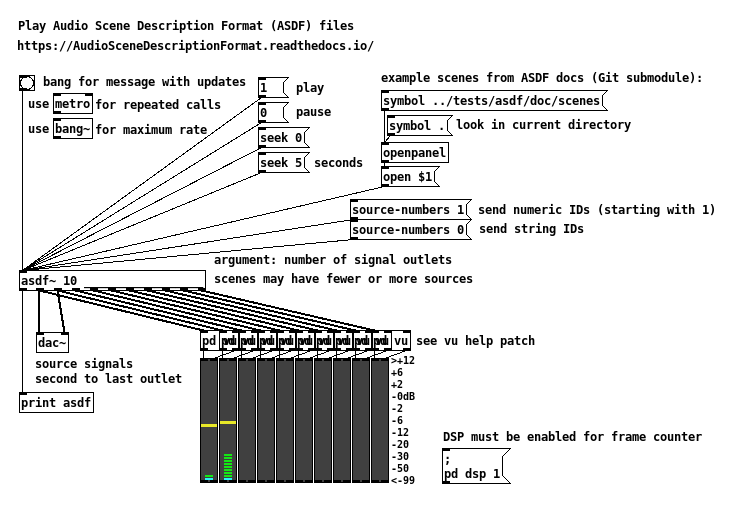
\includegraphics[scale=0.5]{images/asdf-help-pure-data-screenshot}
\caption{Help patch of the \emph{\code{asdf\textasciitilde}} external for Pure Data}
\label{fig:asdf-help-pure-data-screenshot}
\end{figure}

The ASDF library implementation contains\footnote{%
\url{https://github.com/AudioSceneDescriptionFormat/asdf-rust/tree/master/pure-data}}
an \emph{external} for
Pure Data\footnote{\url{https://puredata.info/}}
as a usage example for the C interface.
Figure~\ref{fig:asdf-help-pure-data-screenshot}
shows a screenshot of the external's help patch.
The number of signal outlets has to be provided when creating the external.
Only that number of source signals are provided,
even if more sources are defined in the scene.
Playback of the scene can be started and stopped at any time
and it is possible to \emph{seek} to any point in time in the scene.
The transforms of all sources and the listening position
are not automatically provided at the message outlet,
but they can be triggered at any time
by sending a \emph{bang} message to the external.
However,
all values that have not changed
since the last request
are filtered out.

Given the signals for each source and the corresponding messages
with transform updates,
any means of spatialization available in Pure Data
can be used to auralize a scene.
One possibility are the renderer externals provided by the SSR,
see section~\ref{sec:integration-ssr}.
The messages sent by the ASDF external
happen to be compatible with the SSR externals,
the two just have to be connected.
Both the ASDF and SSR externals can be installed
from Pure Data's built-in package manager.


\section{Visualization}
\label{sec:visualization}

\begin{figure}
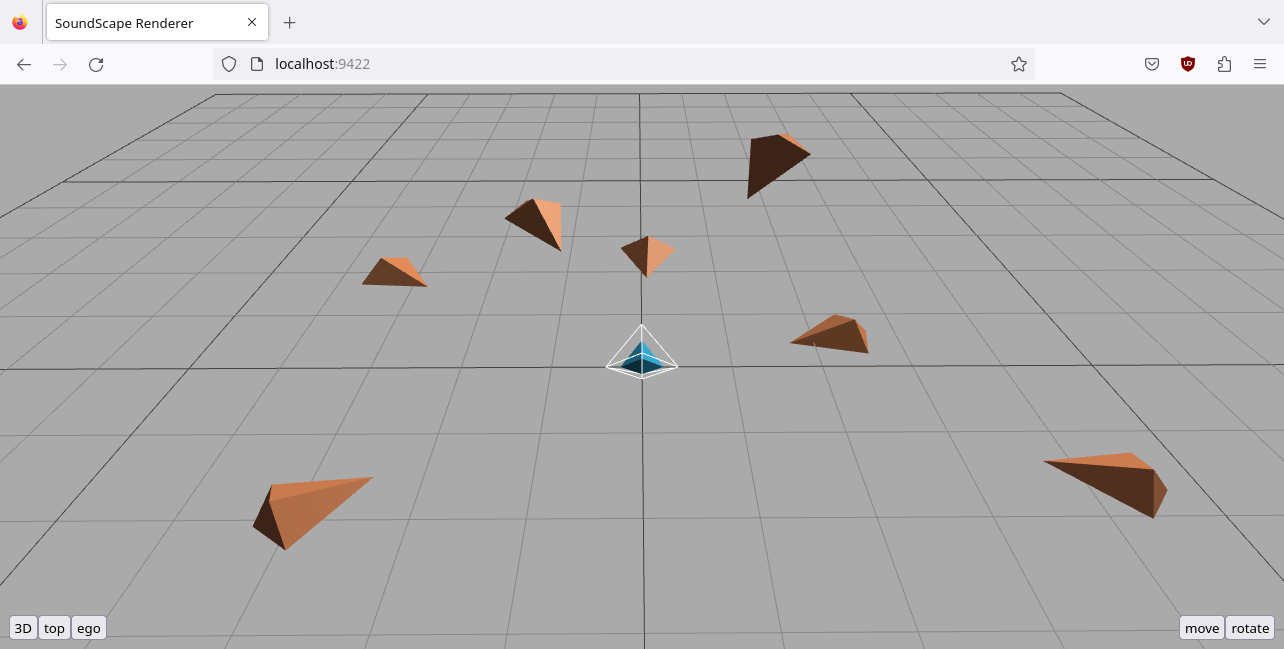
\includegraphics[width=\textwidth]{images/browser-gui-screenshot}
\caption{Screenshot of the browser-based 3D GUI prototype}
\label{fig:browser-gui-screenshot}
\end{figure}

The ASDF is -- as its name suggests --
an audio-only format with no visual aspects.
Nevertheless, it is really helpful for scene authors
to see a visual representation of the sound sources
in the audio scene they are creating.
The ASDF library itself has no capabilities for visualization,
but to aid the development of the ASDF,
a tool for three-dimensional visualization
has been developed for the SoundScape Renderer
(see section~\ref{sec:integration-ssr}).
The tool has been implemented using the
WebGL-based JavaScript library three.js\footnote{\url{https://threejs.org/}}.
More specifically,
it is based on the three.js
editor\footnote{\url{https://threejs.org/editor/}}.
This makes it easy to create a quick prototype
for a three-dimensional user interface
that can be displayed with any modern browser.
The communication with the SSR takes place over the WebSocket protocol,
which is supported by all modern browsers.
A screenshot of web browser displaying an audio scene
is shown in figure~\ref{fig:browser-gui-screenshot}.

The visualization is quite basic and there are many desirable features that are
missing, but it is already possible to get an idea about the three-dimensional
movements of scene objects while the scene is playing.


\section{Example Scenes}

Many minimalistic scenes are available in the ASDF documentation,
see appendix~\ref{sec:asdf}.
Some larger example scenes are available for download from the ASDF development
pages\footnote{%
\url{https://github.com/AudioSceneDescriptionFormat/asdf-example-scenes}}.


\chapter{Conclusion and Future Work}
\label{sec:conclusion}

The previous chapters have shown
the definition of the Audio Scene Description Format (ASDF),
the implementation of a library for loading ASDF files
and its integration into different software for spatial audio reproduction.
All involved programs and libraries are available as open-source software
and for free.
Everyone can use the ASDF to create spatial audio scenes
and the ASDF library and its integrations can be used to play them back.
The software implementation can also be used as a basis for further
experimentation and to prototype features that are currently not implemented.

There has been no systematic evaluation of the format yet,
but everyone is encouraged to try it out and make their own judgement.
As chapter~\ref{sec:existing-formats} has shown,
there are currently no dedicated authoring formats
for spatial audio scenes available.
Therefore, no direct comparison is possible.
From the example scenes in appendix~\ref{sec:asdf} it should be apparent
that the ASDF syntax is more concise and easier to hand-write
than any of the other text-based formats
shown in chapter~\ref{sec:existing-formats}.
The feature set of the ASDF, however,
is very much limited compared to some of the other formats that were mentioned.
The scope of the format is intentionally chosen to be very narrow.
It is focused on the description of
movements and rotation of scene objects over time.
This description is based on different types of \emph{splines},
which are covered in considerable depth in appendix~\ref{sec:splines}.
Nearly everything else is out of scope,
as section~\ref{sec:out-of-scope} describes.

The implementation of the ASDF library covers all features of the format
as currently defined,
but of course additional functionality could be implemented.
One example would be the recording of movements using a tracking system,
followed by a data reduction by means of some kind of \emph{curve fitting},
which would allow to create a high-level declarative description
from a low-level stream of sampled data.

The three-dimensional GUI prototype shown in section~\ref{sec:visualization}
could of course be improved in many ways.
It would be a massive endeavour,
but maybe an application could be implemented that allows
creating and editing trajectories graphically, including the possibility
to animate nested local coordinate systems.
This would also need some kind of elaborate timeline editor
to be able to define the relationships between objects in time.
It is unlikely that such an extensive GUI project would be started
(and more importantly, would lead to a usable program).
More realistically,
some features of the ASDF could probably be improved in order to
simplify the scene authoring process via editing plain text files.
The ASDF has its own issue tracker\footnote{\url{%
https://github.com/AudioSceneDescriptionFormat/asdf/issues}}
where future features can be discussed.

Appendix~\ref{sec:splines} contains a thorough write-up about Euclidean splines
and rotation splines, but it is of course by far not exhaustive,
and more material
-- including more types of splines --
can be added in the future.
Some new findings might even lead to changes in future versions of the ASDF.
For example,
more and better end conditions could be brought forward,
which could replace the end conditions that are currently used in the ASDF.
There is still a lot of old and new literature that has not been incorporated.
Many aspects that might be worth considering in the future
are already mentioned in the issue tracker
for the \emph{splines} project\footnote{\url{%
https://github.com/AudioSceneDescriptionFormat/splines/issues}}.

The ASDF allows the creation of position trajectories and of orientation
trajectories and it can even handle a combination of both.
However, when a scene object or a group of objects moves
along a position trajectory, it does not automatically change its orientation
according to the curvature of the trajectory.
This is a feature that might be desirable for scene authors.

The splines that are currently used in the ASDF
guarantee a continuous change of velocity between spline segments,
but the acceleration vector
-- \ie the second derivative --
is allowed to be discontinuous.
It might be interesting to investigate whether
choosing a different type of spline that guarantees continuity of acceleration
will have any noticeable advantages.

Since all the specifications, software and documentation is publicly available,
it should be easy for anyone who is interested to build upon this work.


\begin{appendices}
\renewcommand{\thechapter}{%
\texorpdfstring{\textsc{\alph{chapter}}}{\Alph{chapter}}}
\renewcommand*{\chapterformat}{\mychapterformat{\mdseries}}

%% headsep=4mm,headheight=6mm
%\newgeometry{inner=25mm,outer=20mm,top=25mm,bottom=15mm}
%% NB: BCOR from the main document is *not* taken into account
%% re-calculate header width
%\fancyhfoffset{0pt}

% This corresponds to parskip=half, see https://tex.stackexchange.com/a/522765/:
\setlength{\parindent}{0pt}
\setlength{\parskip}{.5\baselineskip plus .5\baselineskip}
\setlength{\parfillskip}{1em plus 1fil}

\cleardoubleoddpage
\thispagestyle{empty}
\mbox{}
\vfill
\markboth{}{}%
{\centering
 \normalfont
 \Huge \bfseries \sffamily \appendixpagename\par}%
\vfill

\clearpage
\thispagestyle{empty}
\mbox{}
\vfill
\centerline{\tiny This page intentionally left blank.}
\citeurl{schuetz2010shotcrete}
\vfill
\vfill
\vfill
\clearpage

\chapter{The Audio Scene Description Format (ASDF)}
\label{sec:asdf}

This appendix contains a verbatim copy of the documentation for the ASDF,
which is also available online at
\url{https://AudioSceneDescriptionFormat.readthedocs.io/}.

The example scenes shown in this chapter are available
(including the referenced audio files)
at \url{https://github.com/AudioSceneDescriptionFormat/asdf/}
in the directory \code{doc/scenes/}.
All scenes can be opened and played back with the software
described in sections~\ref{sec:integration-ssr} and~\ref{sec:integration-pd}.

\input{_asdf_build/asdf}


\chapter{Splines}
\label{sec:splines}

This appendix contains detailed information
about many different types of \emph{splines},
including the ones used in the Audio Scene Description Format (ASDF),
as described in appendix~\ref{sec:asdf}.

The following content is a copy of the documentation for the
publicly available Python module \code{splines},
which is also available online at
\url{https://splines.readthedocs.io/}.
In fact, it is recommended to read the online version
instead of the printed version, because the online version contains
a lot of animations which could not be included in this print version.

Nearly all of the content of this appendix has been written using
Jupyter notebooks (see \url{https://jupyter.org/}),
all of which can be downloaded from the sub-directory \code{doc/} at
\url{https://github.com/AudioSceneDescriptionFormat/splines/}
for further study and experimentation.

\input{_splines_build/splines}


\end{appendices}

\backmatter

\printbibliography[title=References,heading=bibintoc]

\end{document}
